\chapter{Analisi di sistemi dinamici lineari tempo invarianti nel dominio di Laplace}
	A pagina \pageref{eq:rapp-matriciale} è stato mostrato come, nel dominio del tempo, la rappresentazione in spazio di stato di un sistema lineare tempo invariante possa essere descritta tramite una notazione matriciale in cui le equazioni di stato assumono una forma $\dot x = Ax+Bu$, mentre le trasformazioni d'uscita diventano $y = Cx+ Du$.
	
	A questo punto per procedere con l'analisi di questo tipo di sistemi è possibile effettuare una trasformazione nel dominio di Laplace, il che si riduce a trasformare completamente la rappresentazione di stato del sistema:
	\[\trasf{\ \begin{cases}
		\dot x = Ax + Bu \\ y = Cx+Du
		\end{cases}} \qquad \Rightarrow\quad \begin{cases}
		\trasf{\dot x(t)} = A\trasf{x(t)} + B\trasf{u(t)} \\
		\trasf{y(t)} = C\trasf{x(t)} + D\trasf{u(t)} 
	\end{cases}\]
	
	Sfruttando a questo punto la proprietà della trasformata della derivata di una funzione per la quale $\trasf{\dot x} = sX(s) - x_0$, allora la rappresentazione in forma di stato rispetto al dominio di Laplace può essere espressa come
	\begin{equation} \label{eq:lti:statolaplace}
		\begin{cases}
			sX(s) - x_0 = AX(s) + BU(s) \\ Y(s) = CX(s) + DU(s)
		\end{cases}
	\end{equation}
	
	\begin{concetto}
		Un \textbf{sistema lineare tempo invariante} può sempre essere descritto sia nel dominio del tempo che nel dominio della variabile di Laplace secondo una notazione matriciale della sua rappresentazione di stato, e nel caso di analisi tramite la teoria del controllo classico tale rappresentazione è mostrata in equazione \ref{eq:lti:statolaplace} (dove in particolare $x_0$ rappresenta lo stato del sistema al tempo $t=0$). \\ Invertendo opportunamente l'equazione di stato e la trasformata di uscita è dunque possibile stabilire il \textbf{movimento di stato} e \textbf{uscita} di un sistema lineare tempo invariante tramite la notazione
		\begin{equation} \label{eq:lti:movimenti}
		\begin{aligned}
			X & = \big(sI-A\big)^{-1} x_0 + \big(sI-A\big)^{-1} BU \\
			Y & = C \big(sI-A\big)^{-1} x_0 + \Big(C\big(sI-A\big)^{-1}B + D\Big)U
		\end{aligned}
		\end{equation}	
	\end{concetto}
	\begin{nota}
		Considerare un sistema come lineare ci permette di utilizzare una rappresentazione di stato in forma matriciale, mentre l'invarianza del sistema permette di stabilire che i coefficienti numerici delle matrici $A,B,C,D$ siano costanti nel sistema (e non dipendano dunque dal tempo).
	\end{nota}
	\begin{nota}
		Nel passaggio dall'equazione \ref{eq:lti:statolaplace} all'equazione \ref{eq:lti:movimenti} si ha l'introduzione del termine $sI$, con $I$ matrice identità, per rendere \textit{confrontabili} le operazioni di somma tra coefficiente scalare $s$ e matrice $A$.
	\end{nota}

	Dall'equazione \ref{eq:lti:movimenti} è dunque possibile stabilire come nel dominio di Laplace sia più \textit{facile} stabilire il movimento di stato e uscita di un sistema, in quanto si tratta di risolvere delle equazioni algebriche in forma matriciale. In particolare al calcolo del movimento libero $ e^{At} x_0 $ è associato il calcolo della matrice $(sI-A)^{-1}$, mentre al calcolo del movimento forzato $\int_0^t e^{A(t-\tau)} B u(\tau)\, d\tau$ è associata l'operazione $(sI-A)^{-1}BU$.
	
	Il \textit{costo} di analizzare il sistema nel dominio di Laplace è che è necessario prima trasformare l'ingresso $u(t)$ e poi anti-trasformare l'uscita $Y(s)$ per poter \textit{visualizzare intuitivamente} il movimento della stessa.
	
\section{Analisi del movimento di stato e uscita} \label{sec:lti:studiomovimenti}
	Dall'equazione \ref{eq:lti:movimenti} è possibile osservare che per determinare i movimenti sia di stato che di uscita è necessario invertire la matrice $sI - A$; in particolare supponendo che la matrice $A$ (sempre quadrata di dimensioni pari all'ordine del sistema) sia composta da elementi $a_{ij}$, allora si può esprimere 
	\[ sI - A = \matrice{s - a_{11} & \dots & -a_{1n} \\ \vdots & \ddots \\ -a_{n1} & & s-a_{nn} }   \]
	
	A questo punto è necessario invertire tale relazione e per fare questo si deve calcolare il \textbf{polinomio caratteristico} della matrice pari a $\varphi(s) = \det(sI-A)$ e calcolare i \textbf{complementi algebrici} $k_{ij}(s)$ della matrice (che risulteranno essere dei polinomi nella variabile $s$ di grado massimo pari a $n-1$):
	\[\big(sI-A\big) ^{-1} = \frac 1 {\varphi(s)} \underbrace{\matrice{k_{11}(s) & \dots & k_{1n}(s) \\ \vdots & \ddots \\ k_{n1}(s) & & k_{nn}(s) }}_K \]
	
	\begin{richiamo}
		Il \textbf{complemento algebrico} $k_{ij}$ (anche detto \textbf{cofattore}) di una matrice quadrata $A$ è calcolato come il determinante della sotto-matrice ottenuta eliminando ad $A$ l'$i$-esima riga e la $j$-esima colonna. Tale coefficiente è moltiplicato per un valore $1$ se la somma $i+j$ è pari, mentre con un valore $-1$ se $i+j$ è dispari.
	\end{richiamo}
	Avendo espresso dunque il termine $(sI-A)^{-1}$ come $\frac 1 {\varphi(s)} K$, ossia come una matrice di polinomi $K$ divisa per il determinante di $sI-A$, è possibile riscrivere il termine $(sI-A)^{-1} B $ dell'equazione \ref{eq:lti:movimenti} come
	\[  \big(sI-A\big)^{-1} = \frac 1 {\varphi(s)} KB = \frac{W(s)}{\varphi(s)} \]
	Anche in questa espressione $W(s)$ rappresenta una matrice di polinomi di ordine massimo pari ad $n-1$ ottenuta come combinazione lineare dei coefficienti di $B$ della matrice dei polinomi di $K(s)$.
	
	Considerando infine il termine $C\big(sI-A\big)^{-1}B + D$, anche questo può essere espresso alla fine come una combinazione lineare di $K(s)$ ottenuta dalle matrici $C$ e $B$ in modo da ottenere una matrice polinomiale $M(s)$ tale da soddisfare
	\[ C\big(sI-A\big)^{-1}B + D = \frac 1 {\varphi(s)} M(s) + D \]
	
	Per praticità scegliendo un sistema dinamico SISO quello che si ottiene è che sia la matrice $M$ che la matrice $D$ risultano essere monodimensionali (ossia appartenenti all'insieme $\mathds R^{1\times 1} = \mathds R$): questo significa che il termine $C\big(sI-A\big)^{-1}B + D$ può essere ridotto ad un polinomio razionale il cui denominatore coincide con il determinante di $sI-A$:
	\[ C\big(sI-A\big)^{-1}B + D = \frac 1 {\varphi(s)} M(s) + D = \frac{N(s)}{\varphi(s)}  \]
	
	\begin{osservazione}
		Il polinomio associato al denominatore $\varphi(s)$ potrà sempre avere grado massimo pari $n$ (dove $n$ è l'ordine del sistema), mentre essendo i polinomi delle matrici $K,W,M$ associati ai complementi algebrici di calcolati partendo da delle sotto-matrici di $sI-A$, il logo grado massimo sarà necessariamente pari a $n-1$ (come già affermato in precedenza). A questo punto considerando quest'ultima relazione riportata per i sistemi SISO si può affermare che $N(s)$ sarà un polinomio di grado al più $n$: in particolare se $D=0$ sicuramente il grado è inferiore (o uguale) a $n-1$ (in quando deriva direttamente da $M(s)$), mentre se $D\neq 0$ può arrivare ad avere un grado pari a quello del denominatore.
	\end{osservazione}
	\begin{concetto}
		Lavorando con sistemi dinamici lineari tempo invarianti, le trasformate associate ai vari ingressi con cui si avrà a che fare avranno sempre la seguenti caratteristiche:
		\begin{itemize}
			\item saranno sempre delle trasformate razionali, ossia sempre esprimibili come un rapporto tra due polinomi:
			\[F(s) = \frac{N(s)}{D(s)} \qquad \textrm{con $N(s),D(s)$ polinomi}\]
			\item il grado del numeratore sarà sempre uguale o minore del grado del denominatore.
		\end{itemize}
	\end{concetto}
	
\section{Stabilità di un sistema}
	
	Dato un sistema dinamico (in questo caso non necessariamente lineare tempo invariante) descritto in forma di stato dalle relazioni $\dot x = f(x,u)$ e $y=g(x,u)$, allora noto lo stato $x_0$ al tempo iniziale e la \textit{storia} degli ingressi $u(t)$, effettuando il passaggio al dominio di Laplace è dunque possibile calcolare il movimento sia dello stato che dell'uscita secondo le espressioni riportate in figura \ref{eq:lti:movimenti}. A questo punto, potendo calcolare tali movimenti, si vuole analizzarne la rispettiva stabilità.
	
	\begin{concetto}
		La \textbf{stabilità} studia la differenza tra un \textbf{movimento nominale} $\hat x, \hat y$ e un \textbf{movimento perturbato} $\tilde x, \tilde y$. In particolare si parla di \textbf{stabilità interna} quando il confronto viene effettuato rispetto al movimento di stato, mentre si parla di \textbf{stabilità esterna} se riferito alle uscite:
		\[ \textrm{stabilità interna: } \|\tilde x(t) - \hat x(t) \| \qquad \textrm{stabilità esterna: } \|\tilde y(t) - \hat y(t) \| \]
	\end{concetto}
	
	La perturbazione del movimento perturbato può essere ottenuta come variazione sia delle condizioni iniziali $\tilde x_0\neq \hat x_0$, sia come variazione degli ingressi $\tilde u(t) \neq \hat u(t)$, tuttavia questo secondo caso generico lo si trascura in quanto è possibile modellare la \textit{storia} degli ingressi pregressi scegliendo un opportuno valore dello stato $\tilde x_0$ al tempo iniziale. In generale le perturbazioni sull'ingresso possono essere sempre ricondotte a perturbazioni sulle condizioni iniziali sullo stato $x_0$ del sistema stesso.
	
	\begin{concetto}
		Analizzando la stabilità di un movimento perturbando lo stato di un sistema permette di determinare 3 tipi di equilibri del moto perturbato rispetto a quello nominale, in particolare
		\begin{itemize}
			\item il movimento è \textbf{instabile} se il moto perturbato diverte da quello nominale ad un valore \textit{infinito};
			\item il movimento è \textbf{semplicemente stabile} se asintoticamente esso converge ad un valore diverso da quello nominale (tuttavia rimane sempre confinato in un intorno del valore perturbato);
			\item il movimento è detto \textbf{asintoticamente stabile} se il moto perturbato converge asintoticamente al valore del movimento nominale.
		\end{itemize}
	\end{concetto}
	
	La classificazione delle proprietà di stabilità del movimento dipende strettamente dal sistema dinamico che si vuole analizzare e dal modello di analisi utilizzato per lo stesso: per esempio un pendolo con attrito risulta essere asintoticamente stabile, mentre un pendolo senza attrito è semplicemente stabile.
	
	\begin{osservazione}
		La stabilità di un movimento è una proprietà locale, ossia solo alcuni movimenti sono stabili e solamente per alcune perturbazioni limitate rispetto allo stato iniziale nominale che si sta considerando. Questo permette di definire infatti la \textbf{regione di attrazione} come l'insieme delle condizioni iniziai per cui il movimento è asintoticamente stabile al valore nominale $\hat x_0$. Quando la regione di attrazione coincide con tutte le possibili condizioni iniziali, si parla allora di \textbf{stabilità asintotica globale}.
	\end{osservazione}
	
	\subsection{Stabilità del movimento per sistemi lineari tempo invarianti}
		Considerando ora il caso di sistemi lineari tempo invarianti, l'equazione \ref{eq:lti:movimenti} permette di descrivere completamente il movimento d'uscita $\|\tilde y(t) - \hat y(t) \|$ (e analogamente il movimento d'uscita). Considerando che per determinare la stabilità si considerano delle perturbazioni sullo stato del sistema e non sugli ingressi, allora è possibile affermare che $\tilde u(t) = \hat u(t)$ il cui risultato si rispecchia anche sulle trasformate $\tilde U(s) = \hat U(s)$. A questo punto è possibile calcolare la variazione tra uscita nominale e perturbata nel dominio di Laplace arrivando al risultato che
		\begin{equation} \label{eq:lti:deltauscita}
			\Delta Y(s) = \hat Y(s) - \tilde Y(s) = C \big(sI-A\big)^{-1}\big(\hat x_0 - \tilde x_0\big) = C\big(sI-A\big)^{-1} \Delta x_0
		\end{equation}
		\begin{concetto} \label{conc:lti:regionetotale}
			Dall'equazione \ref{eq:lti:deltauscita} è possibile osservare che la \textbf{stabilità del movimento d'uscita} di un sistema lineare tempo invariante è associata al \textbf{movimento libero} del sistema; si osserva infatti che la stabilità di questi sistemi non dipende dal particolare movimento considerato, ma assume valenza generale e dunque vale per ogni movimento del sistema.
		\end{concetto}
		Dall'equazione \ref{eq:lti:deltauscita} è possibile osservare che la perturbazione $\Delta x_0$ rappresenta solo un \textit{fattore di scala} della variazione dell'uscita $\Delta Y$, la cui proprietà di stabilità (instabile o asintoticamente/semplicemente stabile) dipende solamente dal termine $C\big(sI-A\big)^{-1}$ e non dalla perturbazione dello stato. Dimostrando dunque che il sistema è asintoticamente stabile, allora la regione di stabilità è globale.
		
		\begin{concetto}
			Lo studio del movimento di stato/uscita perturbato al fronte di cambiamenti/perturbazioni iniziali è equivalente, salvo alcune eccezioni che verranno discusse, allo studio del movimento tramite la risposta del sistema ad un impulso in ingresso.
		\end{concetto}
		Questa affermazione non può essere attualmente dimostrata (ma lo sarà nel seguito), e si basa sul fatto che la trasformata dell'impulso è unitaria per ogni valore del dominio di Laplace $s$. A questo punto per descrivere la stabilità è possibile utilizzare indipendentemente uno dei due metodi: studio della variazione dello stato iniziale o risposta all'impulso:
		\[\textrm{stabilità:} \qquad \Delta Y(s) = C\big(sI-A\big)^{-1} \Delta x_0 \quad \leftrightarrow \quad Y(s) = \Big(C\big(sI-A\big)^{-1}B + D\Big)\cancel{U(s)}\]
		
		In entrambi i casi è possibile osservare che sia la relazione $C\big(sI-A\big)^{-1}$ che $C\big(sI-A\big)^{-1}B + D$ possono essere descritti come un rapporto di un polinomi di numeratore rispettivamente $N(s)$ e $W(s)$ e denominatore uguale e pari a $\varphi(s) = \det(sI-A)$ (rispetto a come visto da pagina \pageref{sec:lti:studiomovimenti}).
		
		Dal punto di vista pratico è più \textit{conveniente} studiare la stabilità come risposta del sistema all'impulso piuttosto che analizzare una variazione dello stato iniziale. Infatti in questo secondo caso la variazione di uscita $\Delta Y$ dipende da $n$ condizioni iniziali coincidenti con l'ordine del sistema, mentre nel caso di risposta all'impulso unitario l'uscita è univocamente determinata dal prodotto matriciale
		\[ \underbrace{\Delta Y(s) = C\big(sI-A\big)^{-1} \Delta x_0}_{\substack{\textrm{1 uscita} \\ \textrm{$n$ condizioni iniziali} }} \qquad \leftrightarrow \qquad \underbrace{Y(s) = C\big(sI-A\big)^{-1}B + D}_{\substack{\textrm{1 uscita} \\ \textrm{condizione iniziale fissata} }}\]

\section{Criteri di stabilità}
	Nel concetto \ref{conc:lti:regionetotale} è affermato che la stabilità di un sistema lineare tempo invariante è una proprietà \textit{strutturale} del sistema stesso, ossia è indipendente dal movimento. A questo punto quello che si vuole stabilire è se, di fatto, il sistema è asintoticamente stabile.
	
	Studiando la risposta all'impulso $Y= C\big(sI-A\big)^{-1} B + D$ è possibile infatti osservare 3 possibili comportamenti del sistema:
	\begin{itemize}
		\item se l'uscita converge al valore nullo allora il \textbf{sistema} è \textbf{asintoticamente stabile};
		\item se l'uscita converge ad un valore reale non nullo, allora il sistema è \textbf{semplicemente stabile};
		\item se l'uscita diverge al valore $\pm \infty$ allora il sistema è detto \textbf{instabile}.
	\end{itemize}	
	
	Potendo scrivere la trasformata dell'uscita $Y(s)$ (per ingressi \textit{canonici}) come un rapporto polinomiale $N(s)/D(s)$, allora applicando il metodo di Heaviside (pag. \pageref{sec:class:heaviside}) è possibile esprimere tale movimento come una combinazione lineare di \textit{elementi più semplici}:
	\[ Y(s) = \frac{N(s)}{D(s)} = \frac A \dots + \frac B \dots + \dots \]
	A questo punto ipotizzando che la trasformata non presenti poli multipli (le radici del denominatore sono \textit{semplici}, non multiple)  e che gli stessi siano reali, allora i vari termini nel dominio del tempo sono associati a degli esponenziali del tipo $e^{-at}$, dove $a$ è il coefficiente costante dei polinomi a denominatore degli elementi semplici di $D(s)$. In particolare il termine $a$ rappresenta l'opposto dei poli della trasformata, e dunque si evince che se i poli sono positivi allora l'esponenziale tende a divergere, per poli nulli l'esponenziale diventa costante e dunque il sistema semplicemente stabile, mentre per poli negativi l'uscita converge al valore nullo e il sistema è asintoticamente stabile.
	\begin{esempio}{: poli e stabilità}
		Si consideri la trasformata $F(s)= \frac{3s^2 - 2 s - 2}{s(s+1)(s-2)} $ i cui poli sono $s=-1,0,2$; applicando la scomposizione di Heaviside è possibile osservare che
		\[ F(s) = \frac{3s^2 - 2 s - 2}{s(s+1)(s-2)}  = \frac 1 s+ \frac 1 {s+1} + \frac  1{s - 2}\]
		\[ \Rightarrow \qquad f(t) = \anti{F(s)} = e^{0t} + \scal (t) e^{-1t} \scal(t) + e^{2t}\scal(t) \]
		Considerando infatti il primo \textit{contributo elementare} pari a $\frac 1 s$ (con coefficiente $a = 0$) a cui è associata l'anti-trasformata $\cancel{e^{0t}} ^{=1} \scal(t)$, si osserva che per $t\rightarrow\infty$ il termine tende al valore unitario. Considerando ora il secondo termine elementare, ossia il polo reale negativo $s=-1$ (cui è associato il coefficiente $a= 1$), si osserva che la sua anti-trasformata $e^{-t}\scal(t)$, per $t\rightarrow \infty$, tende proprio al valore nullo. Al contrario il polo positivo in $s =2$ (coefficiente $a= -2$) presenta anti-trasformata pari a $e^{2t}\scal(t)$ che a tempo infinito diverge.		
	\end{esempio}
	
	Nel caso di poli complessi coniugati distinti, allora la scomposizione di Heaviside determina delle anti-trasformate del tipo $e^{-\sigma t} \sin(\omega t)$, ossia dei segnali (co)sinusoidali smorzati: anche in questo caso la convergenza è associata alla parte reale del polo e in particolare se essa è negativa il sistema è asintoticamente stabile, mentre se essa è positiva il sistema è instabile. Anche nel caso di poli multipli è possibile osservare la convergenza degli elementi in base al \textit{segno} della parte reale delle radici in quanto si osserva che
	\[ \anti{\frac 1 {(s+a)^n}} t^{n-1} e^{-at} \quad \begin{cases}
		\textrm{diverge se il polo è positivo ($a<0$)} \\
		\textrm{converge se il polo è negativo ($a>0$)} 
	\end{cases} \]	
	
	\begin{teorema}{stabilità di sistemi lineari tempo invarianti}  
		
		\texttt{Enunciato:}  { \itshape Dato  un sistema lineare tempo invariante la cui risposta all'impulso è caratterizzata dall'equazione
		\[ Y(s) = C \big(sI-A\big)^{-1} B + D = \frac{N(s)}{\det(sI-A)} = \frac{N(s)}{\varphi(s)} \]  \label{teor:lti:stabilita}
		allora il \textbf{sistema} è \textbf{asintoticamente stabile} se e solo se tutte i \textbf{poli} (radici di $\varphi(s)$) hanno \textbf{parte reale negativa}; il sistema è semplicemente stabile se esiste un solo polo (non multiplo) a parte reale nulla mentre se esiste anche un solo polo a parte reale positiva (o esistono poli a parte reale nulla multipli), il sistema è instabile.}
	\end{teorema}

	In pratica dunque l'analisi di stabilità (esterna) di un sistema lineare tempo invariante si pratica calcolando in primo luogo l'uscita $Y(s)$ come risposta all'impulso, ossia pari a $C \big(sI-A\big)^{-1} B + D$, e poi vi si calcolano i poli che lo compongono.
	
	\begin{esempio}{: stabilità in un sistema lineare tempo invariante} 
		Si consideri il sistema dinamico lineare tempo invariante la cui rappresentazione in forma di stato (nel dominio di Laplace) è dato dalle relazioni
		\[ \dot X= \matrice{-2 & 0 \\ 0 & 4} X + \matrice{1 \\ 1}U \qquad Y = \matrice{1 & 1} X + \matrice{0}U \]
		A questo punto per studiare la stabilità dell'uscita del sistema è sufficiente calcolare la risposta all'impulso dello stesso:
		\begin{align*}
			C\big(sI-A\big)^{-1} B + D & = \matrice{1 & 1} \frac 1 {(s+2)(s-4)} \matrice{s-4 &0 \\ 0 & s+2 }\matrice{1 \\ 1} \\
			& = \matrice{1 & 1} \frac 1 {(s+2)(s-4)} \matrice{s-4 \\ s+2} \\
			&= \frac{2s-2}{(s+2)(s-4)}
		\end{align*}
		Osservando il polinomio $\varphi(s) =(s+2)(s-4)$ a denominatore, si osserva che i suoi zeri (ossia i poli della trasformata dell'uscita $Y$) sono $s_1 = -2$ ed $s_2 = 4$: il primo è a parte reale negativa, e dunque compatibile con l'asintotica stabilità, tuttavia il secondo, essendo a parte reale positiva, determina l'instabilità del sistema dinamico.
	\end{esempio}
	
	\begin{osservazione}
		I poli del denominatore $D(s)$ della trasformata $Y$ di fatto sono associati agli zeri del determinante di $sI-A$, ossia coincidono con le radici del polinomio caratteristico della matrice di stato, o, per essere più precisi, i poli coincidono con gli \textbf{autovalori} della matrice di stato $A$. Va notato però che calcolare la stabilità dell'uscita di un sistema non è consigliato calcolare solamente gli autovalori di $A$: tale metodo infatti può portare a degli errori nell'applicare il teorema i stabilità. Infatti nel calcolo esplicito di $N(s)/D(s)$ è possibile incontrare delle \textit{cancellazioni critiche} tra elementi a numeratore e denominatore che rendono un sistema da instabile a asintoticamente stabile.
	\end{osservazione}
	Nel caso di sistemi di ordine elevato (maggiore di 3) spesso può risultare difficile calcolare i poli dell'uscita $Y(s)$ (e dunque sfruttare il teorema \ref{teor:lti:stabilita}): per questo si devono introdurre dei criteri alternativi per il calcolo della stabilità (indipendenti dal calcolo dei poli).
	
	\subsection{Tabella di Routh}
		Il metodo basato sulla tabella di Routh è un criterio di stabilità basato sull'analisi diretta del polinomio a denominatore della trasformata $Y(s)$ ed è particolarmente efficace quando la fattorizzazione dello stesso non è immediata. In generale il polinomio a denominatore $D(s)$ può essere espresso tramite dei coefficienti generici $d_i$ del tipo
		\[  D(s) = d_0s^n + d_1 s^{n-1} + \dots + d_{n-1}s + d_n \]
		
		\begin{teorema}{condizione di asintotica stabilità} 
			
			Condizione necessaria (ma non sufficiente) affinché un sistema risulti \textbf{asintoticamente stabile} è che tutti i coefficienti $d_i$ del polinomio che compongono il denominatore siano non nulli e di verso concorde. \label{teor:lti:asintotrouth}
		\end{teorema}
		In particolare per polinomi di grado $n=1,2$, tale condizione oltre ad essere necessaria è anche sufficiente. Per polinomi di ordine superiore ($n\geq 3$) la \textbf{condizione sufficiente} per avere asintotica stabilità è che tutti i coefficienti della \textbf{tabella di Routh} siano tutti non nulli e concordi in segno.
		
		\paragraph{Tabella di Routh} Dato un polinomio di grado $n$ (associato al denominatore di una trasformata razionale $Y(s)$), la \textbf{tabella di Routh} (il cui schema generico è mostrato in tabella \ref{tab:lti:routh}) derivante dalla stessa è una tabella di $n+1$ righe così costituite:
		\begin{itemize}
			\item la prima riga contiene i coefficienti $d_i$ con indice $i$ pari (in ordine crescente), mentre la seconda riga contiene i coefficienti di indice dispari;
			\item le $n-1$ righe restanti sono costruite ricorsivamente tramite la seguente relazione: noti i coefficienti di due righe contigue $h_i,k_i$, l'$i$-esimo elemento della riga a loro successiva $l_i$ è determinato dall'equazione
			\[ l_i = - \frac 1{k_1}\det \matrice{h_1 & h_{i+1} \\ k_1 & k_{i+1}} \]
		\end{itemize}
		Gli elementi delle prime due righe che sono necessarie per calcolare gli elementi \textit{discendenti} sono tutti da considerarsi come degli zeri.
		\begin{SCtable}[1][bht]
			\centering
			\begin{tabular}{r | c c c c| }
				prima riga & $d_0$ & $d_2$ & $d_4$ & $\dots$ \\
				seconda riga & $d_1$ & $d_3$ & $d_5$ & $\dots$ \\
				& $\vdots$ \\
				& $h_1$ & $h_2$ & $h_3$ & $\dots$ \\
				& $k_1$ & $k_2$ & $k_3$ & $\dots$ \\
				& $l_1$ & $l_2$ & $l_3$ & $\dots$ \\
			\end{tabular}
			\caption{schema di riferimento della tabella di Routh.} \label{tab:lti:routh}
		\end{SCtable}
		
		\begin{dimostrazione}
			Avendo introdotto il principio di funzionamento della tabella di Routh è ora possibile dimostrare come, per sistemi di ordine 2, la condizione necessaria di coefficienti $d_i$ non nulli concordi (teorema \ref{teor:lti:asintotrouth}) sia anche sufficiente. Considerando il polinomio $D(s) = d_0s^2 + d_1s + d$ composto da coefficienti $d_0,d_1,d_2$ concordi (non nulli), allora le prime due righe della tabella di Routh possono essere considerate nella matrice
			\[ \matrice{d_0 & d_2 \\ d_1 & 0} \]
			
			Essendo il polinomio di ordine 2, allora la tabella di Routh necessiterà solamente di un'altra riga i cui coefficienti $l_i$ possono essere calcolati come
			\[ l_1 = - \frac 1 {d_1}\det \matrice{d_0 & d_2 \\ d_1 & 0} = d_2 \qquad l_2 = - \frac 1 {d_1}\det \matrice{d_0 & 0 \\ d_1 & 0} = 0 \]
			Questo significa che la tabella di Routh presenta coefficienti
			\[ \matrice{d_0 & d_2 \\ d_1 & 0 \\ d_2 & 0} \]
			e dunque essendo $d_0,d_1,d_2$ (elementi della prima colonna della tabella di Routh) tutti concordi e non nulli (per ipotesi iniziale), allora si dimostra che ogni sistema dinamico di ordine 2 (con tale proprietà sui coefficienti) è asintoticamente stabile.
		
		\end{dimostrazione}

	\subsection{Autovalori della matrice di stato e poli di una trasformata}
		In precedenza si era affermato che i poli di una trasformata razionale $Y(s) = N(s)/D(s)$ erano  correlati agli autovalori della matrice di stato $A$ (in quando direttamente determinati dal polinomio caratteristico di tale matrice), tuttavia è necessario fare chiarezza sul considerare gli autovalori per determinare la stabilità o meno di un sistema.
		
		Considerando, per esempio, il sistema rappresentato in forma di stato (nel dominio di Laplace) dalle relazioni
		\[ \dot X= \matrice{0 & 0 \\ 0 & 0} X + \matrice{1 \\ 1}U \qquad Y = \matrice{1 & 1} X + \matrice{0}U \]
		e' possibile osservare che gli autovalori della matrice di stato $A$ sono coincidenti e pari a zero ($\lambda_1 = \lambda_2 = 0$): se tali valori coincidessero con i poli dell'uscita $Y(s)$, allora, per come visto nel teorema \ref{teor:lti:stabilita} (pag. \pageref{teor:lti:stabilita}), si dovrebbe concludere che il sistema è instabile. Tuttavia analizzando la risposta all'impulso si ottiene un risultato diverso, infatti:
		\begin{align*}
			C\big(sI-A\big)^{-1} B + D & = \matrice{1 & 1 } \frac 1 {s^{\cancel{2}}} \matrice{\cancel s & 0 \\ 0 & \cancel s} \matrice{1 \\ 1} + \matrice 0 \\
			& = \frac 1 s \matrice{1 & 1} \matrice{1 \\ 1} = \frac 2 s
		\end{align*}
		Infatti il denominatore dell'uscita $Y$ vale per l'appunto $D(s) = s$, e dunque per lo stesso criterio di stabilità essendo presente una sola radice nulla del denominatore, il sistema può essere considerato come semplicemente stabile.
		
		\begin{concetto}
			In generale è possibile utilizzare gli autovalori della matrice di stato per determinare la stabilità (o meno) di un sistema solamente se gli stessi sono \textit{regolari}, ossia e la loro molteplicità geometrica coincide con quella algebrica: negli altri casi non è possibile asserire alcuna proprietà di stabilità del sistema.
		\end{concetto}
		Per enunciare un criterio di stabilità basato sugli autovalori della matrice di stato analogo a quello visto per le radici di $D(s)$ occorrerebbe analizzare altre proprietà della matrice di stato stessa.
		
		\begin{concetto}
			Gli \textbf{autovalori} determinano di fatto la \textbf{stabilità interna} del sistema, mentre la risposta dell'uscita ad un impulso in ingresso permette di analizzare la \textbf{stabilità esterna} del sistema: in particolare i due movimenti possono essere \textit{diversi} per via della presenza di \textbf{\textit{parti nascoste}} del sistema dinamico che lo rendono \textit{irregolare}.
		\end{concetto}
		\begin{osservazione}
			Per quanto appena affermato, e osservando l'esempio riportato in calce al paragrafo, è possibile affermare che l'instabilità interna non determina necessariamente l'instabilità esterna: il sistema originario infatti era instabile internamente ma semplicemente stabile per quanto riguarda l'uscita.
		\end{osservazione}
		
		\begin{esempio}{: stabilità interna ed esterna}
			Si consideri il seguente sistema dinamico lineare tempo invariante rappresentato in forma di stato nel dominio di Laplace delle equazioni
			\[ \dot X= \matrice{1 & 1 \\ 0 & -3} X + \matrice{1 \\ 1}U \qquad Y = \matrice{0 & 1} X \]
			
			Essendo la matrice di stato $A$ triangolare allora i suoi autovalori coincidono con gli elementi diagonali e dunque sono pari a $\lambda_1 = 1$ e $\lambda_2 = -2$: applicando il teorema di stabilità essendo $\lambda_1$ un elemento a parte reale positiva, allora il movimento di stato (associato alla \textbf{stabilità interna}) è \textbf{instabile}. Al contrario analizzando la risposta all'impulso si può osservare la cancellazione di tale polo, infatti:
			\[ Y(s) = C \big(sI-A\big)^{-1}B = \frac{\cancel{s-1}}{\cancel{(s-1)}(s+2)} = \frac 1 {s+2} \] 
			La radice del denominatore è dunque unica e pari a $s_1 = -2$: utilizzando il teorema di stabilità si evince dunque che il \textbf{sistema} è \textbf{esternamente asintoticamente stabile}.
			
			\vspace{3mm}
			Considerando più nel dettaglio la struttura delle equazioni di stato si determina infatti che
			\[ \begin{cases}
				\dot x_1 = x_1 \\ \dot x_2 = x_1-2x_2 + u \\ y = x_1 + x_2
			\end{cases} \]
			\begin{center}
				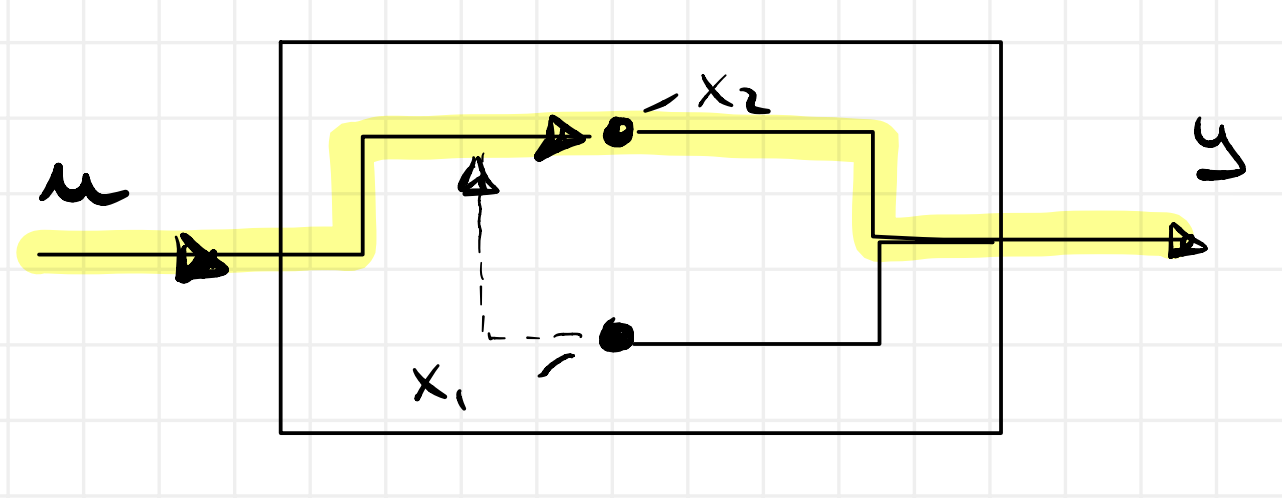
\includegraphics[width=4cm]{sist-nonragg}
			\end{center}
			In questo caso si può affermare che il sistema non è completamente raggiungibile dall'ingresso $u$: gli autovalori della matrice di stato sono in quantità superiore dei poli dell'uscita che risponde all'impulso e dunque l'analisi di stabilità esterna può non coincidere con la stabilità esterna.
			
		\end{esempio}
	
	\subsection{Osservabilità di un sistema dinamico}
		Si consideri il sistema dinamico mostrato in figura \ref{sist-inoss} composto da due masse che possono scorrere sul piano. L'attuatore idraulico (o il sensore di elongazione) permettono dunque di determinare uno spostamento (o misurarlo rispettivamente) relativo tra le due masse $m_1,m_2$, ma non permettono di determinare la posizione assoluta delle stesse.	
	
		\figura{5}{3}{sist-inoss}{sistema composto da due carrelli in cui $m_1$ è collegato a telaio da una molla, mentre $m_2$ è collegato ad $m_1$ tramite una molla e un attuatore/sensore (evidenziato in giallo).}{sist-inoss}
		
		Questo è un esempio pratico di \textbf{sistema non completamente raggiungibile/osservabile}: analizzando la rappresentazione in forma di stato del sistema dinamico ci si accorge infatti che l'ordine del denominatore $D(s)$ è minore dell'ordine del sistema dinamico di partenza, il che implica che nel processo di analisi dell'impulso è stata commessa una cancellazione.
		
		\vspace{3mm}
		
		La sola ispezione delle equazioni di stato non sempre permette di individuare se il sistema è completamente raggiungibile o osservabile; per effettuare tale analisi è necessario ricorrere a strumenti quali:
		\begin{itemize}
			\item il confronto dell'ordine del polinomio a denominatore $D(s)$ con l'ordine del sistema (se il primo ha grado inferiore del secondo, allora sono state effettuate delle cancellazioni critiche);
			\item utilizzare dei test specifici di raggiungibilità ed osservabilità; tali metodi (che non verranno trattati) si basano sulla formulazione della matrice di raggiungibilità $R = f(A,B)$ e dalla matrice di osservabilità $O = f(A,C)$.
		\end{itemize}
		
		
	\subsection{Osservazioni e BIBO stabilità}
		Dato un sistema dinamico lineare tempo invariante, e ipotizzando che lo stesso sia completamente raggiungibile/osservabile, allora la stabilità del sistema stesso è una proprietà strutturale, ossia è indipendente dalla rappresentazione che si fa dello stesso (una scelta di diverse variabili di stato deve necessariamente portare alla stessa conclusione sui risultati).
		
		Per questo tipo di sistemi l'asintotica stabilità in uscita dipende solamente dall'ingresso $u(t)$, e non dalle specifiche condizioni iniziali $x_0$ del sistema: tale asserzione è particolarmente desiderata nelle applicazioni reali in quanto si \textit{eliminano} così gli effetti di disturbo (il movimento di equilibrio dipende solo dall'ingresso, e non dallo stato).
		
		Sistemi lineari tempo invarianti asintoticamente stabili sono caratterizzati dall'avere uno e un solo punto di equilibrio (unico): gli autovalori della matrice di stato sono tutti a parte reale negativa. Essendo garantita la possibilità di calcolare l'inversa (per il fatto che $\det A \neq 0$), allora si può determinare l'equilibrio del sistema ed essendo per ingressi costanti l'uscita asintotica, allora l'uscita tende al movimento di equilibrio.
		
		\begin{concetto}
			Un sistema è dunque detto \textbf{BIBO stabile} se e solo se ad ogni suo ingresso limitato (\textit{Bounded Input}) corrisponde un'uscita limitata (\textit{Bounded Output}).
		\end{concetto}
		A questo punto è possibile dimostrare che condizione necessaria e sufficiente affinché un sistema lineare tempo invariante sia BIBO stabile è che i poli dell'uscita ottenuta da uno scalino in ingresso abbia poli siano tutti a parte reale positiva (ossia che il sistema sia esternamente asintoticamente stabile).
		
	\subsection{Stabilità per sistemi non lineari}
		In generale il concetto di \textit{stabilità} di un sistema dinamico è associato al \textit{movimento dell'uscita} e non al \textit{sistema} stesso (per sistemi lineari spesso tale concetto può essere confuso in quanto la stabilità è una proprietà del sistema, ma non vale in generale per sistemi non lineari). A questo punto per analizzare il tipo di stabilità dei movimenti dell'uscita di sistemi non lineari è possibile utilizzare diversi strumenti matematici; verranno qui accennati due metodi per lo studio del movimento di equilibrio di un sistema per questo tipo di sistemi.
		
		\paragraph{Metodo indiretto di Lyapunov} Il \textbf{metodo indiretto di Lyupanov} si basa sullo studio della stabilità del movimento dell'uscita del sistema linearizzando lo stesso nell'intorno del punto di equilibrio. Facendo così è possibile trasformare il sistema non lineare in un sistema lineare che può essere analizzato con le metodologie accennate in precedenza.
		
		Se analizzando il sistema linearizzato si conclude che lo stesso è semplicemente stabile, allora non è possibile asserire alcuna conclusione sulla stabilità del sistema non lineare originario (potrebbe infatti essere che, nella realtà, il sistema sia asintoticamente stabile oppure instabile).
		
		\paragraph{Metodo grafico per sistemi scalari} Per sistemi non lineari scalari, ossia di ordine $n=1$, è possibile analizzarne la stabilità tramite un metodo grafico. Facendo riferimento per esempio all'equazione di stato $\dot x = f(x,\overline u)$ in figura \ref{graf-scal} associata all'ingresso costante $\overline u$, è possibile osservare che i punti di equilibrio sono quelli che annullano la derivata $\dot x$ (indicati con $\overline x_1,\overline x_2,\overline x_3$).		
			
		\figura{6}{1}{graf-scal}{grafico di riferimento per l'analisi grafica di stabilità di un sistema non lineare.}{graf-scal}
		
		Per studiare la stabilità dei punti di equilibrio determinati è possibile pensare di perturbare lo stato $x$ nell'intorno di uno dei punti di equilibrio $\overline x_i$. Osservando il verso della derivata $\dot x$ è infatti possibile predire lo spostamento dello stato: per esempio nel caso di derivata positiva (indicata dalle frecce gialle nel diagramma di riferimento) la variabile di stato perturbata tenderà ad andare verso destra, mentre se la derivata è negativa (in blu) lo stato tenderà a spostarsi verso sinistra.
		
		A questo punto è possibile osservare che il punto di equilibrio $\overline x_1$ è asintoticamente stabile in quanto una perturbazione (non troppo accentuata) dello stato verrà \textit{riportata} per l'effetto della derivata al punto di equilibrio. Al contrario perturbando i punti $\overline x_2,\overline x_3$ lo stato, per effetto della derivata, tenderà a divergere dal punto di equilibrio: il sistema è dunque instabile.
		
		\begin{esempio}{: stabilità di un sistema non lineare scalare}
			Si consideri il sistema dinamico non lineare di ordine unitario la cui rappresentazione di stato è
			\[ \begin{cases}
				\dot x = - x^3 + u \\ y = x
			\end{cases} \]
			Volendo studiare la stabilità per un ingresso costante $\overline u = 0$, risolvendo l'equazione di stato si ottengono 3 soluzioni coincidenti per lo stato di equilibrio del sistema $\overline x_{1,2,3} = 0$. Volendo provare a determinare il tipo di stabilità del sistema lineare è possibile pensare di \textbf{linearizzare} la rappresentazione di stato del sistema, ossia determinando le matrici $A,B,C,D$ come visto a pagina \pageref{sec:intro:linearizzazione}; in particolare essendo il sistema scalare ogni matrice sarà di dimensione $1\times 1$, ossia un coefficiente numerico:
			\[ A = \left. \pd f x\right|_{\overline x,\overline u} = - 3x^2 \Big|_{\substack{x = 0 \\ u = 0}} = 0 \qquad
			B = \left. \pd f u\right|_{\overline x,\overline u} = 1 \Big|_{\substack{x = 0 \\ u = 0}} = 1 \]
			\[ C = \left. \pd g x\right|_{\overline x,\overline u} = 1 \Big|_{\substack{x = 0 \\ u = 0}} = 1 \qquad 
			D = \left. \pd g u\right|_{\overline x,\overline u} = 0 \Big|_{\substack{x = 0 \\ u = 0}} = 0 \]
			
			Per procedere con lo studio della stabilità del sistema è necessario determinare la risposta allo scalino del sistema che è determinata dall'equazione
			\[ C\big(sI-A\big)^{-1} B +  D = \frac 1 s \]
			A questo punto l'unico polo dell'uscita $Y(s)$ è posto nella posizione $s=0$, e dunque se il sistema fosse lineare significherebbe che il sistema è \textbf{semplicemente stabile}. Tuttavia essendo il sistema non lineare, allora non è possibile affermare con precisione il tipo di stabilità. 
			\begin{multicols}{2}
			Analizzando \textbf{graficamente} invece l'equazione di stato risulta evidente immediatamente che nella realtà il sistema è \textbf{asintoticamente stabile}: spostando infatti lo stato dalla sua condizione di equilibrio $\overline x=0$, il \textit{segno} della derivata tenderà sempre a riportarlo verso il punto di equilibrio (che è per questo asintoticamente stabile).
			
			\begin{center}
				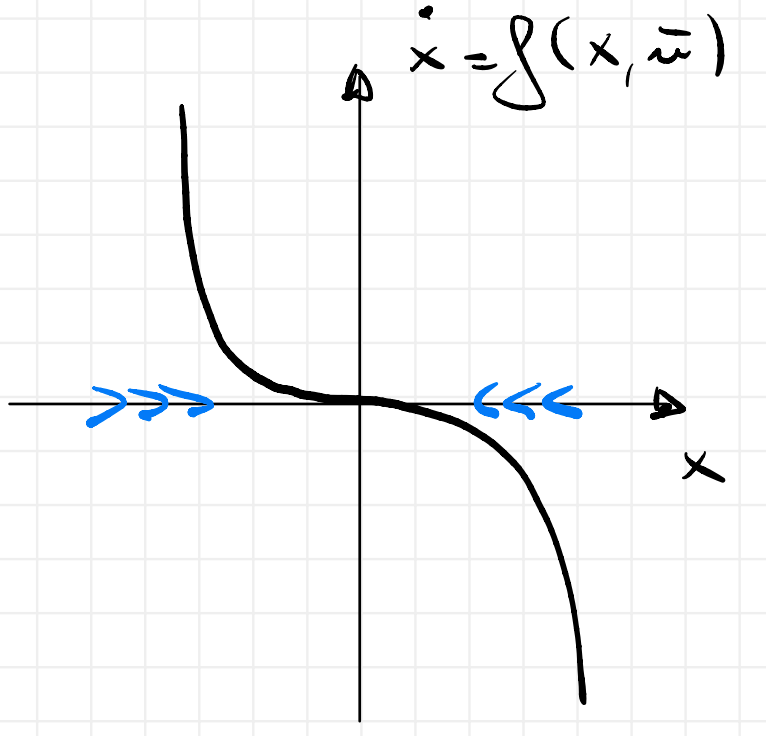
\includegraphics[width=3cm]{graf-scal-es}
			\end{center}
		\end{multicols}
		
		\end{esempio}
		
\section{Funzione di trasferimento}
	In precedenza si er descritto il movimento d'uscita di un sistema dinamico lineare nel dominio di Laplace, osservando che (come nel dominio del tempo) esso prevedeva sia una componente di movimento libero che di movimento forzato (eq. \ref{eq:lti:movimenti}, pag. \pageref{eq:lti:movimenti}).
	\begin{concetto} Considerando ora solamente la parte di movimento forzato, ossia imponendo che lo stato iniziale $x_0$ sia nullo, è possibile determinare la cosiddetta \textbf{funzione di trasferimento} $G(s)$ di un sistema dinamico tempo invariante
		\begin{equation}
			Y(s) = \underbrace{\Big(C\big(sI-A\big)^{-1}B+D\Big)}_{G(s)} U(s)
		\end{equation}
	\end{concetto}
	La funzione di trasferimento dunque permette di correlare direttamente l'uscita $Y$ di un sistema (nel dominio di Laplace) con la sua uscita; considerando il movimento forzato espresso nel dominio del tempo come
	\[ y(t) = C\int_0^t e^{A(t-\tau)}Bu(\tau)\, d\tau + Du(t) \]
	appare evidente che la relazione ingresso-uscita mediante funzione di trasferimento è molto più \textit{facile} da calcolare rispetto alla rispettiva relazione nel dominio del tempo.
	
	Nella pratica è possibile determinare la funzione di trasferimento di un sistema lineare attraverso due metodologie:
	\begin{itemize}
		\item supponendo di conoscere il modello analitico del sistema, ossia note le matrici $A,B,C,D$ che lo descrivono, è possibile determinare \textit{a priori} analiticamente la funzione di trasferimento applicando la definizione:
		\[ G(s) = C\big(sI-A\big)^{-1}B+D \]
		\item se non si conosce il modello del sistema ma è tuttavia possibile calcolare le trasformate di un ingresso arbitrario e la rispettiva uscita, si può determinare la funzione di trasferimento per inversione del modello:
		\[ G(s) = \frac{Y(s)}{U(s)}\]
	\end{itemize}
	

	\begin{concetto}
		La \textbf{funzione di trasferimento} rappresenta di fatto la \textbf{risposta all'impulso} di un sistema dinamico: considerato infatti che $\trasf{\imp(t)} = 1 $ per ogni valore $s$, allora calcolando l'uscita del sistema si osserva che essa coincide con la funzione di trasferimento:
		\[ Y(s) = G(s) \cancel 1 \qquad \textrm{se } U(s) = \trasf{\imp(t)} \]
	\end{concetto}	

	Nel caso particolare di sistema lineare SISO la funzione di trasferimento è di fatto una trasformata razionale (rapporto di due polinomi), mentre se il sistema è MIMO $G(s)$ rappresenta di fatto una \textbf{matrice di trasferimento}, ossia una \textit{collezione} di trasformate razionali caratterizzate dall'avere il polinomio a denominatore comune; in questo caso l'elemento $g_{ij} \in G(s)$ rappresenta la funzione di trasferimento sussistente tra l'$i$-esima uscita e il $j$-esimo ingresso (vigendo il principio di sovrapposizione degli effetti, l'uscita complessiva del sistema sarà determinata dalla somma dei contributi di tutti gli ingressi).
	
	\vspace{3mm} E' anche possibile osservare che l'analisi di stabilità esterna fin'ora analizzata di fatto si basava sul determinare la posizione dei poli nel piano complesso della funzione di trasferimento $G(s)$ del sistema dinamico; per come già visto nel caso di sistemi lineari tempo invarianti completamente raggiungibili/osservabili tali poli coincidono con gli autovalori della matrice di stato $A$ e la funzione di trasferimento è una proprietà \textit{strutturale} del sistema, ossia indipendente dalla scelta delle variabili di stato per descrivere il problema.
	
	\subsection{Parametrizzazioni della funzione di trasferimento}
		La stessa funzione di trasferimento $G(s)$ può essere espressa in diverse formulazioni alternative. Essa infatti (ai fini di questo corso) è sempre descritta come il rapporto tra due polinomi $N(s)$ e $D(s)$: tali polinomi possono infatti essere descritti, in maniera equivalente, tramite una \textit{forma fattorizzata} e una \textit{forma polinomiale} come nell'esempio che segue
		\[ \underbrace{(s+1)(s+2)}_\textrm{fattorizzata} = \underbrace{s^2+3s + 2}_\textrm{polinomiale} \]
	
		\begin{concetto}
			Sfruttando l'idea di \textit{riscrivere} in maniera alternativa i polinomi, in equazione \ref{eq:lti:parametrizzazione} è possibile osservare 3 rappresentazioni analoghe una funzione di trasferimento, in particolare sono rappresentante la \textbf{forma polinomiale} (a), la \textbf{forma fattorizzata di Nyquist} (b) e \textbf{forma fattorizzata di Bode} (c).
			\begin{subequations} \label{eq:lti:parametrizzazione}
			\begin{align}
				G(s) & = \frac{\beta_ns^n + \beta_{n-1}s^{n-1} + \dots + \beta_1 s + \beta_0}{s_n + \alpha_{n-1}s^{n-1}+ \dots + \alpha_0} \\
				& = \frac{\rho}{s^g} \frac{ \prod_i \big(s + z_i\big) \prod_i \big( s^2 + 2\eta_i\alpha_i s+ \alpha_i^2 \big) }{ \prod_i \big(s + p_i\big) \prod_i \big( s^2 + 2\xi_i\omega_i s+ \omega_i^2 \big) } \\
				& = \frac{\mu}{s^g} \frac{ \prod_i \big(\tau_is + 1\big) \prod_i \left( \frac{s^2}{\alpha_i^2} + 2 \frac{\eta_i}{\alpha_i} s + 1  \right) } { \prod_i \big(T_is + 1\big) \prod_i \left( \frac{s^2}{\omega_i^2} + 2 \frac{\xi_i}{\omega_i} s + 1  \right) }
			\end{align}
			\end{subequations}
		\end{concetto}
	
		La forma polinomiale (\ref{eq:lti:parametrizzazione}a) di fatto è caratterizzata da $2n-1$ coefficienti associati ai parametri $\alpha_i,\beta_i$ dei termini del polinomio. Questa forma risulta essere di poca utilità pratica in quanto è difficile determinare la stabilità del sistema dinamico in quanto non è immediato determinare i poli della funzione di trasferimento: per questo motivo sono più \textit{comode} le forme fattorizzate di Nyquist e di Bode.
		
		In entrambe le forme fattorizzate è possibile osservare la presenza del parametro $g$: esso prende il nome di \textbf{grado} del sistema dinamico e rappresenta il numero di poli (se positivo) o zeri (se negativo) presenti nell'origine. \\
		Per quanto riguarda la forma fattorizzata di Nyquist (\ref{eq:lti:parametrizzazione}b) si indica con  $\rho$ la \textbf{costante di trasferimento}, con $z_i\neq 0$ i valori opposti degli zeri reali della funzione di trasferimento, mentre $p_i \neq 0$ rappresentano l'opposto dei poli reali (termini associati alla produttoria \textit{a sinistra} di numeratore e denominatore). Le produttorie \textit{a destra} di numeratore/denominatore determinate dai coefficienti $\eta_i/\xi_i$ e $\alpha_i/\omega_i$ sono utilizzate per rappresentare invece i poli complessi coniugati. In particolare i termini $\eta_i,\xi_i$ (il cui modulo è sempre inferiore o pari a 1) rappresentano gli \textbf{smorzamenti del polo}, mentre i termini $\alpha_i,\omega_i > 0$ rappresentano le \textbf{pulsazioni naturali}.\\
		La forma fattorizzata di Bode (\ref{eq:lti:parametrizzazione}c) è molto simile a quella di Nyquist, in quanto si può pensare come la sua \textit{ normalizzazione}; il termine $\mu$ prende il nome di \textbf{guadagno} mentre i termini $\tau_i = 1 / z_i$ e $T_i = 1 / p_i$ rappresentano le \textbf{costanti di tempo} di zeri e poli rispettivamente.
		
		Nota la costante di trasferimento $\rho$ nella forma di Nyquist di può ricavare il guadagno nella forma di Bode tramite la relazione
		\[ \mu = \rho \frac{\prod_i z_i \prod\alpha_i^2}{\prod_i p_i \prod\omega_i^2} \] 
		
		\paragraph{Poli (e zeri) complessi coniugati} Si consideri un polo di smorzamento $\xi$ e pulsazione naturale $\omega$ (ma il ragionamento è analogo per gli zeri di una funzione di trasferimento), allora la rappresentazione nella forma di Nyquist e Bode vale rispettivamente
		\[ \underbrace{s^2 + 2 \xi \omega s + \omega^2}_\textrm{Nyquist} \qquad \leftrightarrow \qquad \underbrace{\frac{s^2}{\omega^2} +2 \frac \xi \omega s + 1 }_\textrm{Bode} \]
		 In entrambi i casi calcolando le radici di tali espressioni si ottengono i valori
		 \[ s_{1,2} = \underbrace{- \xi \omega}_\textrm{Re} \pm i\underbrace{ \omega \sqrt{1 - \xi^2}}_\textrm{Im} \]
		 Le due radici sono infatti dei numeri complessi composti da una parte reale pari a $-\xi\omega$ e da una parte immaginaria di valore $\omega \sqrt{1-\xi^2}$. Volendo dare un \textit{significato rappresentativo} (come in figura \ref{complessi}) alle due grandezze, i poli complessi coniugati possono essere descritti nel piano dei numeri immaginari come dei punti (descritti da vettori) distanti $\omega$ dal centro del piano e con angolo $\theta$ (calcolato come in figura \ref{complessi}) tale che
		 \[ \xi = \cos\theta \]
		 
		\figura{6}{1}{complessi}{rappresentazione nel piano dei numeri immaginari di un polo complesso coniugato.}{complessi}
		Essendo i poli complessi coniugati, determinato un polo l'altro può essere ottenuto specchiando il primo rispetto all'asse dei numeri reali. Poli con smorzamento positivo sono posizionati nel semipiano a parte reale negativa, mentre smorzamenti negativi sono nel semipiano destro a parte reale positiva.
		 
	\subsection{Sistemi a ritardo di tempo}
		\begin{concetto}
			Sono detti \textbf{sistemi a ritardo di tempo} tutti quei sistemi che \textit{ritardano} l'uscita; in particolare l'uscita $y(t)$ è pari all'ingresso $u$ in ritardo di un coefficiente $\tau$, ossia $y(t) = u(t-\tau)$. Sfruttando la proprietà di traslazione nel dominio del tempo (eq. \ref{eq:class:proptraslazionetempo}, pag. \pageref{eq:class:proptraslazionetempo}) la funzione di trasferimento di questo sistema può dunque essere espressa come
			\begin{equation}
				G(s) = e^{-\tau s}
			\end{equation}
		\end{concetto}
		Questo tipo di sistema dinamico sarà l'unico \textit{non canonico} nel corso: la sua trasformata infatti non è razionale ma è una funzione trascendente (cosa che in generale può dare problemi nell'analizzare il problema).	
	
\section{Studio del legame ingresso-uscita}
	Avendo determinato la funzione di trasferimento $G(s)$ di un sistema dinamico tempo invariante tramite la forma fattorizzata di Nyquist/Bode (eq. \ref{eq:lti:parametrizzazione}), si vuole ora cercare di interpretare il \textit{significato} dei vari elementi che compongono le parametrizzazioni (poli, zeri, smorzamenti, pulsazioni...) e come gli stessi influenzano i sistemi dinamici. Particolarmente importante sarà dunque analizzare due tipi di risposta: quella ad un ingresso a scalino (per determinare le proprietà di transitorio del sistema) e quelle di un ingresso sinusoidale.
	
	\subsection{Risposta allo scalino}
		La risposta allo scalino di un sistema dinamico è interessante da analizzare in quanto permette di studiare il comportamento di un sistema che passa da una condizione di quiete ad un'altra condizione di quiete diversa (chiaramente affinché ciò si verifichi si deve garantire l'asintotica stabilità del sistema che si sta analizzando). In particolare essendo il sistema lineare è sufficiente calcolare la risposta del sistema allo scalino unitario in quanto ogni altro tipo di scalino può essere determinato tramite il principio di sovrapposizione degli effetti.
		
		\begin{concetto}
			La \textbf{risposta allo scalino} viene utilizzata per determinare molte delle proprietà \textit{salienti} del transitorio di un sistema dinamico, in particolare:
			\begin{itemize}
				\item il \textbf{valore iniziale} $y_0$ (ed eventualmente le sue derivate $\dot y_0,\ddot y_0,\dots$) dell'uscita del sistema;
				\item il \textbf{valore asintotico} $y_\infty$ dell'uscita, ossia il valore cui tende la stessa per $t\rightarrow \infty$;
				\item il \textbf{tempo di assestamento} $t_a$, ossia dopo quanto tempo la risposta del segnale può essere approssimata al valore asintotico, e l'eventuale \textbf{periodo} $T$ di oscillazioni del sistema;
				\item l'eventuale \textbf{sovra-elongazione} (\textit{overshoot}) $s_\%$ dell'uscita, definita come il rapporto percentuale tra uscita massima $y_{max}$ nella fase transitoria e valore asintotico:
				\[ s_\% = \frac{|y_{max} - y_\infty|}{y_\infty} 100 \]
			\end{itemize}
		\end{concetto}
		Nel seguito verranno dunque discusse alcune casistiche di funzioni di trasferimento \textit{semplici} ma i cui risultati verranno estesi a carattere più generale
		
		\subsubsection{Sistemi del primo ordine con un polo nell'origine}
			Si consideri il sistema di ordine unitario la cui parametrizzazione della funzione di trasferimento è $G(s) = \dfrac \mu s$, dove $\mu$ è il guadagno del sistema; questo sistema presenta dunque un solo polo nell'origine (mentre non sono presenti zeri). A questo punto per studiare la risposta allo scalino è necessario moltiplicare $G(s)$ per la trasformata dell'ingresso dello scalino, ossia
			\[ Y(s) = G(s) U(s) = \frac \mu s \frac 1 s = \frac{\mu}{s^2} \]
			
			Essendo verificate le condizioni iniziali del teorema \ref{teor:valiniziale} del valore iniziale (pag. \pageref{teor:valiniziale}) è possibile calcolare l'uscita $y_0$ nel dominio del tempo tramite la relazione
			\[ y_0 = \lim_{s\rightarrow\infty}s \, Y(s) = \lim_{s\rightarrow\infty}\cancel{s}  \frac{\mu}{s^{\cancel{2}}} = 0 \]
			Osservato che l'uscita iniziale è nulla è possibile pensare di calcolarne la derivata: sfruttando la relativa proprietà (eq. \ref{eq:class:derivata}, pag. \pageref{eq:class:derivata}) è possibile affermare infatti che $\trasf{\dot y} = s Y(s) - y(0)$. Noto che $y(0)=y_0=0$ (ed essendo ancora la trasformata razionale) è possibile applicare ulteriormente il limite del valore iniziale e dunque
			\[ \dot y_0 = \lim_{s\rightarrow \infty} s \big(sY(s) - y_0\big) = \lim_{s\rightarrow\infty} \cancel{s^2} \frac{\mu}{\cancel{s^2}} = \mu \]
	
			Per quanto riguarda la risposta asintotica è possibile invece utilizzare il teorema \ref{teor:valfinale} del valore finale (pag. \pageref{teor:valfinale}): essendo la trasformata razionale e con poli a parte reale nulla allora vale che
			\[ y_\infty = \lim_{s\rightarrow 0} s\,Y(s) = \lim_{s\rightarrow 0} \frac \mu s = \infty \]
			
			Questi risultati in realtà sono \textit{attendibili} rispetto a quello che ci si aspettava dal sistema: anti-trasformando l'uscita $Y(s)$ si osserva infatti che
			\[ y(t) = \anti{F(s)} = \mu \anti{\frac 1 {s^2}} = \mu \ramp(t) \]
			Osservando infatti il grafico dell'uscita $y(t)$ nel dominio del tempo (fig. \ref{scal1-a}) si osserva che l'uscita parte da valore nullo e con una pendenza pari a $\mu$ diverge a $\infty$. Essendo il sistema non asintoticamente stabile (il polo in $s=0$ afferma che il sistema è semplicemente stabile) allora esso non potrà essere neanche BIBO stabile: ad un ingresso limitato quale lo scalino è associata infatti un'uscita non limitata.
			
			\figura{5}{1}{scal1-a}{risposta allo scalino di un sistema con funzione di trasferimento $G(s) = \mu / s$ con $\mu = 10$.}{scal1-a}
	
			\begin{concetto}
				Facendo riferimento all'esempio appena mostrato è possibile affermare che, a carattere generale, se il tipo $g$ della funzione è positivo non nullo (in questo caso essendo presente un polo nell'origine si ha $g=1$) allora la risposta allo scalino del sistema non si assesta a nessun valore di regime.
			\end{concetto}
	
		\subsubsection{Sistema del primo ordine con polo non nell'origine}
			Si consideri ora un sistema di ordine $n=1$ con un polo a parte reale negativa non nulla (in modo da garantire l'asintotica stabilità del sistema) la cui funzione di trasferimento fattorizzata in forma di Bode vale
			\[ G(s) = \mu \frac 1{Ts + 1} \qquad \xrightarrow[\textrm{scalino}]{\textrm{risposta allo}} \quad Y(s) = G(s) U(s) =  \frac \mu {s\big(Ts + 1\big)} \]
			
			Calcolata dunque la trasformata $Y(s)$ della risposta allo scalino applicando il teorema del valore iniziale è possibile calcolare che $y_0=0$, mentre $\dot y_0 = \mu / T$ (come nel caso di polo nell'origine il valore iniziale è nullo, tuttavia la derivata dell'uscita risulta divisa per la costante di tempo $T$ del polo). Applicando invece il teorema del valore finale si osserva che
			\[ y_\infty = \lim_{s\rightarrow 0} s\,Y(s) = \lim_{s\rightarrow 0} \frac \mu{s\big(Ts + 1\big)} = \mu \]
			\begin{nota}
				E' possibile applicare il teorema del valore finale solamente perché si era ipotizzato inizialmente che il polo fosse a parte reale negativa (ossia deve essere che $T>0$), altrimenti non sarebbero rispettate le ipotesi di applicabilità.
			\end{nota}
			Effettuando l'anti-trasformazione con il metodo di Heaviside è possibile risalire all'uscita $y(t)$  del sistema nel dominio del tempo, e in particolare
			\[ y(t) = \anti{\frac \mu{s\big(Ts + 1\big)}} = \mu \left(1 - e^{-t/T}\right)\]
			Osservando la rappresentazione grafica dell'uscita (figura \ref{scal1-b}) è possibile osservare che $y(t)$ non presenta oscillazioni (e dunque il relativo periodo è pari a zero) e come anche l'elongazione percentuale $s_\%$ sia nulla.
			\figura{5}{1}{scal1-b}{risposta allo scalino di un sistema con funzione di trasferimento $G(s) = \frac \mu {Ts + 1}$ con parametri $\mu = 10$ e $T=2$.}{scal1-b}
			
			A questo punto non resta altro che calcolare il tempo di assestamento $t_a$ del sistema, ossia quel valore che, scelta una tolleranza $\varepsilon$, verifica la relazione
			\begin{equation} \label{eq:lti:tolleranza}
				\big|y(t_a) - y_\infty\big| \leq \varepsilon \, y_\infty
			\end{equation}
			
			\begin{concetto}
				Impostata una tolleranza $\varepsilon = 0.01$ (ossia $1\%$) tramite calcolo esplicito della relazione \ref{eq:lti:tolleranza} è possibile determinare che il \textbf{tempo di assestamento} di una funzione di trasferimento ad un solo polo che vale
				\begin{equation} \label{eq:lti:tempo1polo}
					t_a = 4.6T \approx 5T
				\end{equation}
			\end{concetto}
			Questo significa che ad un tempo $t$ pari a 5 volte la costante di tempo $T$ del polo l'errore che si commette a considerare l'uscita asintotica rispetto a quella reale è inferiore all'$1\%$ e dunque, a livello ingegneristico, è possibile considerare che il sistema è a regime.
			\begin{osservazione}
				Il tempo di assestamento non dipende dal guadagno $\mu$ del sistema, ma solamente dalla costante di tempo $T$ del polo.
				\begin{center}
					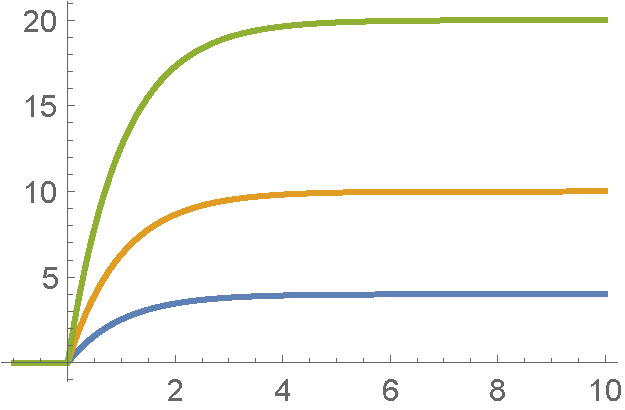
\includegraphics[width=5cm]{scal1-c}
				\end{center}
				In figura sono infatti riportate 3 funzioni di trasferimento per le quali la costante di tempo è uguale e pari a $T=1$, mentre il guadagno è variabile ($\mu = 3,10,20$): è possibile osservare che in tutti i casi dopo il tempo $t_a = 5T=5$ la risposta può essere considerata pressoché stazionaria.
			\end{osservazione}
			
			Rappresentando nel piano dei numeri immaginari i poli si osserva che la loro posizione nell'asse dei numeri reali dipende dalla costante di tempo $T$ e vale $-1/T$ (figura \ref{lentoveloce}): questo significa che dati due sistemi per cui $T_1 > T_2$ allora il primo sistema sarà più lento (per via del maggiore tempo di assestamento) e dunque il polo associato sarà più vicino all'origine. 
			
			\figura{5}{1}{lentoveloce}{posizione nel piano complesso di due poli con costanti di tempo $T_1>T_2$.}{lentoveloce}
			
			Questo significa che per avere dei sistemi dinamici con tempo di assestamento molto basso è necessario \textit{spostare} i poli il più possibile lontano (\textit{verso sinistra}) dal centro del piano dei numeri complessi, diminuendo il più possibile la parte reale, il che può essere fatto diminuendo il più possibile la costante di tempo (in figura \ref{scal1-d} è mostrato un esempio).
		
			\figura{5}{1}{scal1-d}{risposta allo scalino di un sistema con funzione di trasferimento $G(s) = \frac \mu {Ts + 1}$ con guadagno $\mu = 10$ e costanti di tempo $T=1$ (funzione arancione) e $T = 3$ (blu).}{scal1-d}
		\subsubsection{Sistema del secondo ordine a poli coincidenti}
			Si consideri ora un sistema del secondo ordine a poli coincidenti (a costante di tempo $T >0$ in modo da garantire che i poli siano a parte reale negativa) la cui funzione di trasferimento e relativa risposta allo scalino sono descritte dalle trasformate razionali
			\[ G(s) =  \frac \mu{\big(Ts + 1\big)^2} \qquad \xrightarrow[\textrm{scalino}]{\textrm{risposta allo}} \quad Y(s) = G(s) U(s) = \frac \mu{s\big(Ts + 1\big)^2} \]
			
			Applicando il teorema del valore iniziale si calcola che sia $y_0$ che la sua derivata $\dot y_0$ sono nulle, mentre il primo termine non nullo è la derivata seconda dell'uscita che risulta valere $\ddot y_0 = \mu / T^2$.
			\begin{osservazione}
				A livello intuitivo è dunque possibile iniziare a pensare che il numero di poli della funzione di trasferimento è associato all'ordine del primo valore di derivata che risulterà non essere nulla al tempo iniziale.
			\end{osservazione}
			Avendo ipotizzato che il polo multiplo della funzione di trasferimento sia a parte reale negativa è dunque possibile applicare il teorema del valore finale e osservare che l'uscita asintotica (come nel caso di un solo polo a parte reale negativa) vale $y_\infty = \mu$. \\			
			A questo punto è possibile anti-trasformare l'uscita $Y(s)$ tramite il metodo di Heaviside che determina l'uscita
			\[ y(t) = \anti{ \frac \mu{s(Ts + 1)^2}} = \mu \left( 1- e^{-t/T} - \frac t T e^{-t/\tau} \right) \] 
			\begin{nota}
				La trasformata razionale dell'uscita $Y(s)$ è di ordine 3 e la scomposizione di Heaviside associata a tale funzione vale
				\[ Y(s) = \frac As + \frac B{Ts+1} + \frac C{\big(Ts+1\big)^2} \]
				Determinando dunque i coefficienti $A$ (che risulterà valere $\mu$), $B$ ($-\mu$) e $C$ ($-\mu/T$) l'anti-trasformata è composta da $y(t) = A \scal(t) + Be^{-t/T} + Ct e^{-t/T}$.					 
			\end{nota}
			
			\figura{5}{1}{scal2-a}{risposta allo scalino di un sistema con funzione di trasferimento $G(s) = \frac \mu {(Ts + 1)^2}$ con parametri $\mu = 10$ e $T=2$.}{scal2-a}
			
			Graficando l'uscita del sistema dinamico (figura \ref{scal2-a}) si osserva che la funzione non è periodica ($y$ è composta da un solo esponenziale) e non si ha neanche sovra-elongazione (in quanto $y_{max} = y_\infty$). Invertendo l'equazione \ref{eq:lti:tolleranza} per l'uscita nel dominio del tempo appena determinata, considerando una tolleranza $\varepsilon = 1\%$ allora si dimostra che il tempo di assestamento del sistema vale
			\begin{equation}\label{eq:lti:tempo2poli}
				t_a = 6.64T
			\end{equation}
			
			Confrontando questo risultato con quello ottenuto per i sistemi ad un polo (eq. \ref{eq:lti:tempo1polo}) è possibile osservare che, a parità di costante di tempo $T$, i sistemi a polo multiplo sono più lenti (figura \ref{scal2-b}).
			\figura{5}{1}{scal2-b}{risposta allo scalino di un sistema ad un polo (arancione) e due poli coincidenti (azzurro) con costanti di tempo e guadagno eguali.}{scal2-b}
		
		\subsubsection{Sistema a due poli reali distinti}
			Considerando ora un sistema a due poli reali distinti (a costanti di tempo $T_1,T_2>0$ in modo da garantire l'asintotica stabilità del sistema) allora è possibile esprimere la sua funzione di trasferimento e relativa risposta allo scalino tramite le trasformate razionali
			\[ G(s) =  \frac \mu{\big(T_1s + 1\big) \big(T_2s + 1\big) } \qquad \xrightarrow[\textrm{scalino}]{\textrm{risposta allo}} \quad Y(s) = G(s) U(s) = \frac \mu{s\big(T_1s + 1\big) \big(T_2s + 1\big) } \]
			Tramite i teoremi di valore iniziale e finale si osserva che, come nel caso precedente, $y_0 = \dot y_0 = 0$ e la risposta asintotica $y_\infty$ è costante e pari al guadagno $\mu$; l'unica variazione che si può osservare è nel calcolo della derivata seconda del valore iniziale che risulta valere $\ddot y_0 = \dfrac \mu {T_1T_2}$. \\
			A questo punto anti-trasformando con il metodo di Heaviside l'uscita $Y(s)$ del sistema può essere espressa nel dominio del tempo arrivando alla conclusione che
			\[ y(t) = \mu \Big(  1 - \underbrace{\frac{T_1}{T_1-T_2} e^{-t/T_1}}_{\substack{\textrm{esponenziale} \\ \textrm{associato} \\ \textrm{a $T_1$}}} + \underbrace{\frac{T_2}{T_1-T_2} e^{-t/T_2} }_{\substack{\textrm{esponenziale} \\ \textrm{associato} \\ \textrm{a $T_2$}}} \Big) \]
			Il risultato dell'uscita può essere rappresentata nel dominio del tempo tramite il grafico in figura \ref{scal2-c}. Si osserva che essendo la risposta esponenziale allora non si ha periodicità nel segnale e anche la sovra-elongazione $s_\%$ è nulla. Per quanto riguarda il tempo di assestamento è possibile osservare che, considerando per esempio $T_1>T_2$, il tempo di assestamento del sistema dovrà sempre essere compresa tra il valore minimo associato ad una funzione di trasferimento con polo singolo di costante $T_1$ e il valore massimo rappresentato da un sistema a polo doppio con medesima costante di tempo.
						
			\figura{5}{2}{scal2-c}{risposta allo scalino di un sistema con funzione di trasferimento $G(s) = \frac \mu {(T_1s + 1)(T_2s+1)}$ con parametri $\mu = 10$, $T_1=3$ e $T_2 = 1.5$ (in azzurro); in arancione è rappresentata la zona rispetto al quale il comportamento del sistema a due poli distinti può appartenere.}{scal2-c}
			
			Nel caso limite in cui $T_2 = T_1$ infatti il comportamento del sistema coincide con quello di una funzione di trasferimento a due poli reali coincidenti e per cui il tempo di assestamento vale $t_a = 6.64 T$ (eq. \ref{eq:lti:tempo2poli}). Al contrario nel caso in cui $T_2 \ll T_1$ l'esponenziale associato a $T_2$ si \textit{esaurisce} molto rapidamente (raggiunge la stazionarietà prima del polo associato a $T_1$) e dunque il tempo di assestamento può essere approssimato alla funzione di trasferimento ad un unico polo di tempo $T_1$ e dunque con tempo di assestamento $t_a =5T_1$.
			
		\subsubsection{Sistema a due poli complessi coniugati}
			Si consideri un sistema la cui funzione di trasferimento presenta due poli complessi coniugati di pulsazione $\omega$ e smorzamento $\xi$ che, rappresentato in forma di Bode, assume la forma
			\[ G(s) = \frac \mu {\dfrac{s^2}{\omega^2} + 2 \dfrac \xi \omega s + 1} \] 
			
			Dall'analisi tramite il teorema del valore iniziale e finale è possibile stabilire le caratteristiche iniziali dell'uscita pari per cui $y_0 = \dot y_0 = 0$ e $\ddot y_0 = \mu \omega^2$.	L'uscita asintotica, anche in questo caso, risulta valere $y_\infty = \mu$. \\
			In questo caso tuttavia, analizzando il sistema tramite la scomposizione di Heaviside, si osserva che l'uscita presenta una componente sinusoidale; anti-trasformando $Y(s)$ si osserva infatti che
			\[ y(t) = \anti{\frac 1 {s \left( \frac{s^2}{\omega^2} + 2 \frac \xi \omega s + 1 \right)}  } = y(t) = \mu \left[ 1 - \frac 1 {\sqrt{1-\xi^2}} e^{-\xi\omega t} \sin\big(\omega \sqrt{1-\xi^2} + \theta\big) \right] \]
			
			L'uscita $y(t)$, mostrata in figura \ref{scal3-a}, presenta dunque una \textbf{componente oscillatoria} il cui \textbf{periodo} può essere calcolato come
			\begin{equation}
				T = \frac{2\pi}{\omega \sqrt{1-\xi^2}} = \frac{2\pi}{\textrm{Im}}	
			\end{equation}
			Tale periodo dipende dunque solamente dal valore della parte immaginaria del sistema (maggiore è la parte immaginaria, più piccolo risulterà essere il periodo).
			\begin{osservazione}
				Con questa considerazione è possibile considerare i sistemi a poli puramente reali (per cui $\textrm{Im} = 0$) come delle funzioni oscillanti con periodo $T\rightarrow \infty$ verificando che
				\[ T = \lim_{\textrm{Im}\rightarrow 0} \frac{2\pi}{\textrm{Im}} = \infty  \]
			\end{osservazione}
			
			\figura{5}{1}{scal3-a}{risposta allo scalino di una funzione di trasferimento di guadagno $\mu = 2$ a due poli complessi coniugati di pulsazione $\omega = 1$ e smorzamento $\xi = 0.3$.}{scal3-a}
			Questo tipo di sistema è anche caratterizzato dalla presenza di una \textbf{sovra-elongazione} il cui valore percentuale dipende dal rapporto tra parte reale e immaginaria secondo la relazione
			\begin{equation}
				s_\% = 100 \exp \left(-\frac{\xi \omega}{\sqrt{1-\xi^2}}\right) = 100 e^{-\textrm{Re} / \textrm{Im}}
			\end{equation}
			
			\begin{nota}
				Nel caso estremo in cui lo smorzamento è unitario ($\xi = 1$), allora i poli sono puramente immaginari (senza parte reale): in questo caso l'uscita non converge e inizia ad oscillare tra un valore compreso tra 0 e $2\mu$  come si può osservare nella figura che segue.
				\begin{center}
					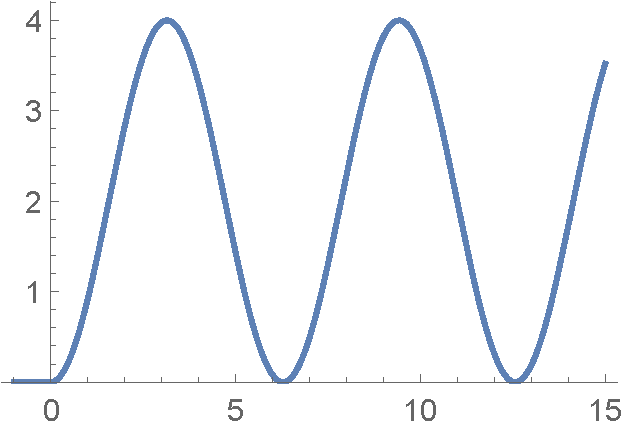
\includegraphics[width=5cm]{scal3-b}
				\end{center}
			\end{nota}
			Il \textbf{tempo di assestamento} associato all'esponenziale convergente può dunque essere calcolato e dipende solamente dalla parte reale del polo; in analogia al caso di polo unico puramente reale il tempo di assestamento viene calcolato come
			\begin{equation}
				t_a = \frac 5 {\xi \omega} = \frac 5 {\textrm{Re}}
			\end{equation}
			
		\subsubsection{Zero reale nell'origine}
			Fino ad ora si è osservato l'effetto che la posizione dei poli ha nel calcolo delle caratteristiche salienti delle funzioni di trasferimento di sistemi lineari: si vuole analizzare ora invece come gli zeri influenzano la risposta (anche se le considerazioni che trarremo non saranno a carattere generale come nel caso dell'analisi dei poli).
			
			Considerando un primo esempio di funzione di trasferimento con zero reale nell'origine, ossia di tipo $g = -1$, e con un solo polo stabile (con costante di tempo $T>0$) allora $G(s)$ può essere espressa come
			\[ G(s) = \frac{\mu s}{Ts+1} \qquad \xrightarrow[\textrm{scalino}]{\textrm{risposta allo}} \quad Y(s) = G(s) U(s) = \frac \mu {Ts+1} \]
			Applicando il teorema del valore iniziale si osserva che lo stesso non parte più da un valore nullo, ma dal valore $y_0 = \mu/T$; anche il valore finale, tramite l'utilizzo del relativo teorema, si dimostra essere diverso dai casi precedenti e convergente al valore $y_\infty = 0$; questo fatto può essere intuitivamente dimostrato considerando che il polo nell'origine $s$ coincide con l'operatore derivata (eq. \ref{eq:class:derivata}, pag. \pageref{eq:class:derivata}): derivando la risposta ad un polo (figura \ref{scal1-b}) e osservando che la stessa tende asintoticamente ad una costante, allora la sua derivata è nulla. 
			\begin{concetto}
				L'effetto generale di introdurre un zero nell'origine è quello di annullare la risposta asintotica del sistema.
			\end{concetto}
			Anti-trasformando l'uscita con il metodo di Heaviside è possibile calcolare la risposta del sistema nel dominio del tempo secondo l'espressione
			\[ y(t) = \anti{\frac{\mu s}{(Ts+1)s}} = \frac \mu T e^{-t/T} \]
			Facendo riferimento alla rappresentazione dell'uscita in figura \ref{scal4-a} è possibile osservare come lo zero non cambi le proprietà del transitorio: in particolare esso è determinato ancora dalle caratteristiche del polo a parte reale negativa e dunque con tempo di assestamento $t_a = 5T$.
			
			
			\figura{5}{1}{scal4-a}{risposta allo scalino di una funzione di trasferimento del tipo $\frac{\mu s}{Ts+1}$ con guadagno $\mu = 2$ e costante di tempo $T=2$.}{scal4-a}
			
		\subsubsection{Zero reale non nell'origine}
			Si consideri una funzione di trasferimento del primo ordine con polo a parte reale negativa ($T>0$ per garantire l'asintotica stabilità del sistema) e con uno zero con costante di tempo $\tau \neq 0$ (in questo caso non è necessario imporre il \textit{segno} della posizione del polo in quanto non appartiene alle specifiche dei criteri di stabilità) e dunque nella forma
			\[ G(s) = \mu \frac{\tau s + 1}{Ts+1}  \qquad \xrightarrow[\textrm{scalino}]{\textrm{risposta allo}} \quad Y(s) = G(s) U(s) = \mu \frac{\tau s + 1}{s(Ts+1)}\]
			A questo punto dall'analisi dei teoremi del valore iniziale e finale è possibile calcolare sia il valore iniziale, che risulta valere $y_0  \mu \tau/T$, che il valore asintotico $y_\infty =\mu$ (che torna dunque a coincidere con il guadagno della funzione di trasferimento). Anti-trasformando con Heaviside si ottiene dunque la funzione $y$  pari a 
			\[y(t) = \anti{\mu \frac{\tau s + 1}{s(Ts+1)}} = \mu \left(1 + \frac{\tau - T}T e^{-t/T}\right)  \]
			Anche in questo caso gli zeri reali non influiscono sul transitorio (il cui tempo di assestamento è determinato dal polo e dunque $t_a = 5T$), tuttavia è possibile osservare come la costante di tempo $\tau$ cambia il valore iniziale $y_0$ dell'uscita: in particolare per $\tau <0$ (zero a parte reale positiva) l'uscita parte da un valore negativo, per $0<\tau<T$ l'uscita parte da un valore compreso tra 0 e $\mu$ mentre per $\tau > T$ il valore iniziale $y_0$ è maggiore del guadagno e si ha dunque un fenomeno di sovra-elongazione (figura \ref{fig:lti:sist1zero}).
			
			\begin{figure}[bht]
				\centering
				\begin{subfigure}{0.325\linewidth}
					\centering
					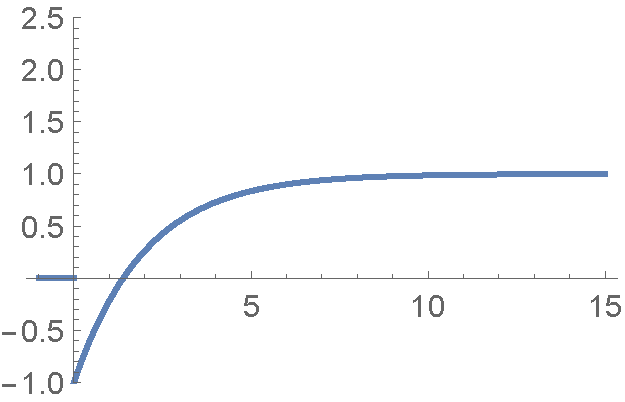
\includegraphics[width=4cm]{scal4-b} \caption{}
				\end{subfigure}
				\begin{subfigure}{0.325\linewidth}
					\centering
					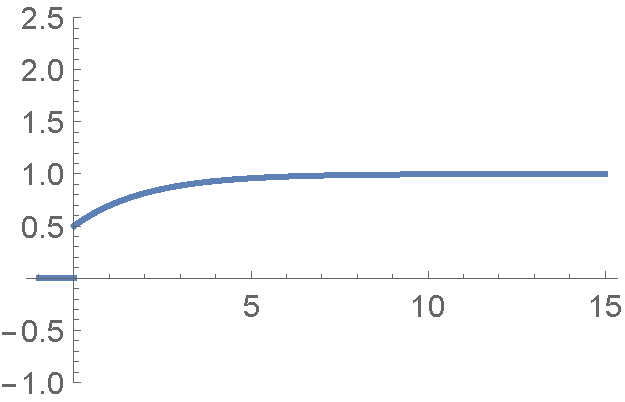
\includegraphics[width=4cm]{scal4-c} \caption{}
				\end{subfigure}
				\begin{subfigure}{0.325\linewidth}
					\centering
					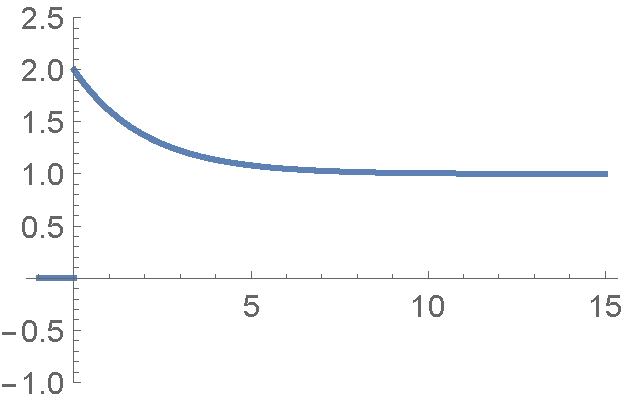
\includegraphics[width=4cm]{scal4-d} \caption{}
				\end{subfigure}
				\caption{risposta allo scalino di una funzione di trasferimento del tipo $\mu \frac{\tau s + 1}{Ts+1}$ con guadagno $\mu = 1$, costante di tempo $T=2$ e costanti di tempo degli zeri che cambiano: $\tau = -2$ (a), $\tau = 1$ (b) e $\tau = 4$ (c).} 
				\label{fig:lti:sist1zero}
			\end{figure}
		
		\subsubsection{Sistemi di ordine 2 con uno zero}
			Si consideri il sistema asintoticamente stabile ($T_1,T_2>0$) con zero non nell'origine la cui funzione di trasferimento vale
			\[ G(s) = \mu \frac{\tau s + 1}{\big(T_1s +1\big)\big(T_2s+1\big)} \qquad \xrightarrow[\textrm{scalino}]{\textrm{risposta allo}} \quad Y(s) = \mu \frac{\tau s + 1}{s\big(T_1s +1\big)\big(T_2s+1\big)} \]
			Dall'analisi tramite i teoremi del valore iniziale e finale si conclude che $y_0=0$ mentre $\dot y_0 = \mu \dfrac{\tau}{T_1T_2}$, mentre l'uscita asintotica rimane pari al guadagno $y_\infty = \mu$.
			\begin{concetto}
				A livello generale l'ordine della prima derivata di $y(t)$ non nulla nell'origine dei tempi coincide con il grado relativo della funzione di trasferimento, ossia tra la differenza del numero di poli e il numero di zeri di $G(s)$.
			\end{concetto}
			
			Anti-trasformando con il metodo di Heaviside è dunque possibile stabilire l'uscita in funzione del tempo:
			\[ y(t) = \anti{\mu \frac{\tau s + 1}{s\big(T_1s +1\big)\big(T_2s+1\big)}} = \mu \left( 1 - \frac{T_1-\tau}{T_1-T_2} e^{-t/T_1} + \frac{T_2-\tau}{T_1-T_2}e^{-t/T_2} \right) \]
			A livello intuitivo non è possibile capire quale sia il comportamento dell'uscita in funzione delle varie costanti di tempo $T_1,T_2,\tau$, tuttavia utilizzando i grafici (in figura \ref{fig:lti:sist2zero}, nella pagina seguente) è possibile osservare le seguenti proprietà:
			\begin{itemize}
				\item[a)] se lo zero è a parte reale positiva (ossia con $\tau <0$) allora si ha il fenomeno della cosiddetta \textbf{\textit{risposta inversa}} dove inizialmente l'uscita tende a valori negativi prima di riportarsi al valore del guadagno (più vicino è il polo dall'origine, più l'effetto sarà pronunciato);
				
				\item[b)] se lo zero è a parte reale negativa ma si trova più vicino all'origine dei poli (e dunque $\tau > T_1,T_2$) allora il sistema va incontro ad un fenomeno di sovra-elongazione che è tanto maggiore quanto più lo zero si avvicina all'origine dei numeri complessi;
				
				\item[c, d)] se lo zero determina una costante di tempo $\tau$ confrontabile con i valori $T_1,T_2$, allora l'effetto sarà quello di una \textit{cancellazione} e il comportamento viene approssimato ad una funzione di trasferimento ad un solo polo (complementare rispetto a quello cancellato);
				
				\item[e)] se lo zero ha una costante di tempo compresa tra quella dei poli ($T_2 < \tau < T_1$) allora il comportamento dell'uscita sarà compresa tra la risposte dei sistemi a un solo polo reale con costanti $T_1$ e $T_2$ rispettivamente;
				
				\item[f)] se lo zero si trova più \textit{lontano rispetto all'origine} dei poli (ossia per $\tau < T_1,T_2$) allora il comportamento dell'uscita convergerà al caso di una funzione a due poli reali in $T_1,T_2$ (senza effetto del polo).
				
			\end{itemize}
			
			\begin{figure}[p]
				\centering
				\begin{subfigure}{0.48\linewidth}
					\centering
					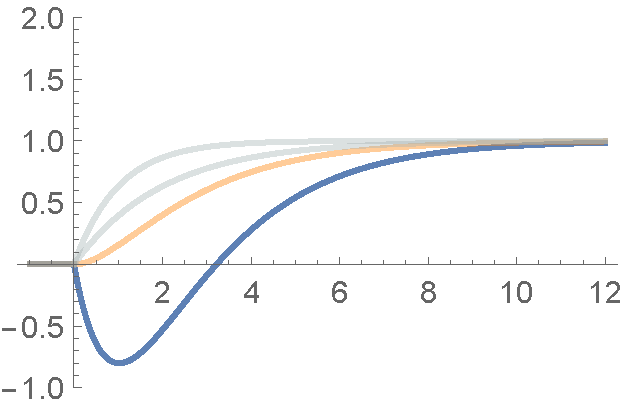
\includegraphics[width=6cm]{scal5-a} \caption{}
				\end{subfigure}
				\begin{subfigure}{0.48\linewidth}
					\centering
					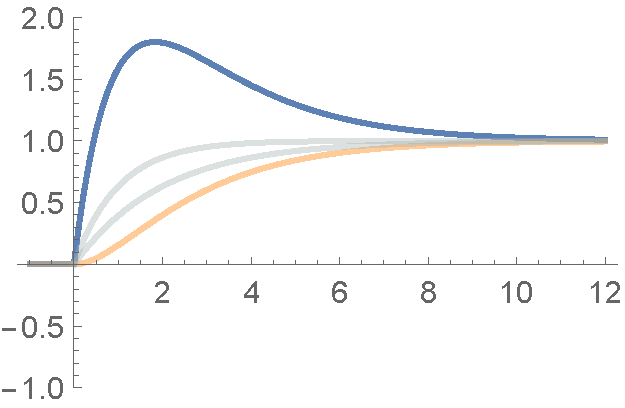
\includegraphics[width=6cm]{scal5-b} \caption{}
				\end{subfigure}
				\begin{subfigure}{0.48\linewidth}
					\centering
					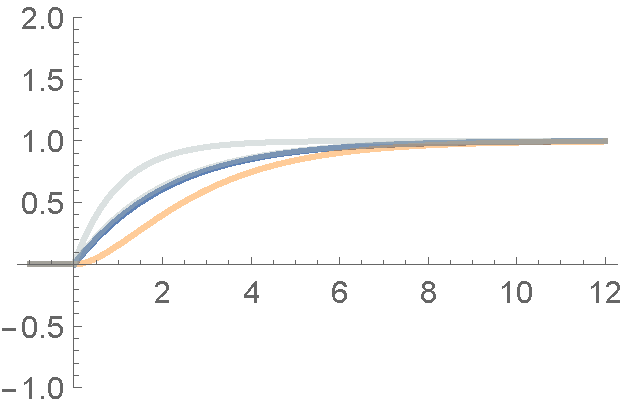
\includegraphics[width=6cm]{scal5-c} \caption{}
				\end{subfigure}
				\begin{subfigure}{0.48\linewidth}
					\centering
					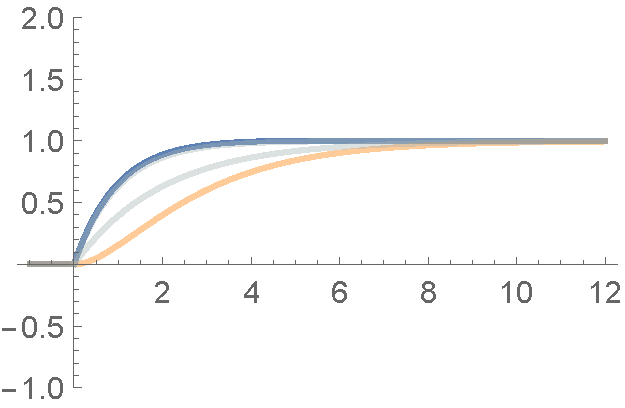
\includegraphics[width=6cm]{scal5-d} \caption{}
				\end{subfigure}
				\begin{subfigure}{0.48\linewidth}
					\centering
					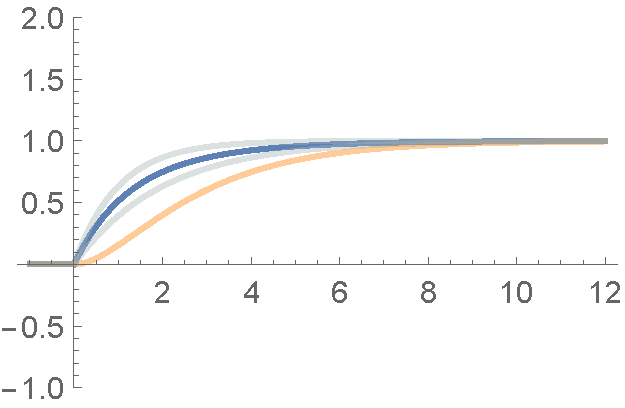
\includegraphics[width=6cm]{scal5-e} \caption{}
				\end{subfigure}
				\begin{subfigure}{0.48\linewidth}
					\centering
					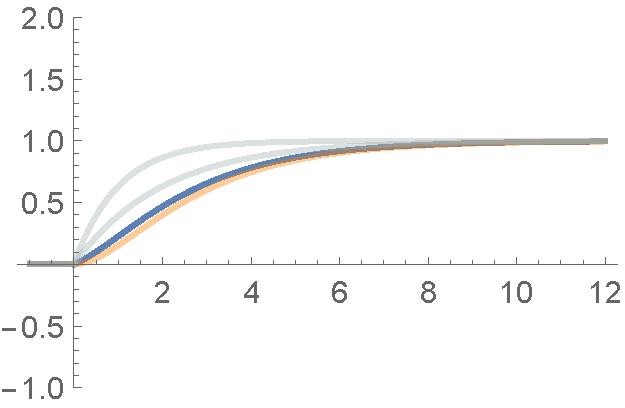
\includegraphics[width=6cm]{scal5-f} \caption{}
				\end{subfigure}
			
				\caption{risposta allo scalino di una funzione di trasferimento del tipo $\mu \frac{\tau s + 1}{(T_1s+1)(T_2s+1)}$ con guadagno $\mu = 1$, costanti di tempo $T_1 = 2$ e $T_1 = 1$. In arancione è mostrato il comportamento della funzione composta dai soli poli reali, mentre in grigio è mostrata la risposta dei sistemi ad un solo polo (di costanti $T_1$ e $T_2$ rispettivamente). In blu sono mostrate le risposte per valori $\tau = -4$ (a) cui è associato il fenomeno della risposta inversa, $\tau = 6$ (b) cui è associato il fenomeno della sovra-elongazione, $\tau = 0.9 \approx T_2$ (c) e  $\tau = 2.1 \approx T_1$ (d) cui è associato l'effetto di cancellazione, $\tau=1.5$ (e) e $\tau =0.3$ (f).}
				\label{fig:lti:sist2zero}
			\end{figure}
		
		\subsubsection{Effetto degli zeri sulla risposta allo scalino}
			A questo punto è possibile riassumere in maniera sintetica gli effetti che l'aggiunta degli zeri provoca sul sistema, in particolare:
			\begin{itemize}
				\item zeri nell'origine ($G(s)$ con tipo $g\leq -1$) annullano la risposta asintotica del sistema (considerando che la stessa sia pari ad una costante);
				\item gli zeri \textit{destri} (a parte reale positiva) determinano il fenomeno della risposta inversa, mentre gli zeri vicini all'asse immaginario determinano un fenomeno di sovra-elongazione;
				\item gli zeri vicini ad un polo tendono a \textit{mascherarne} l'effetto, ossia come se vi fosse una cancellazione critica nel sistema;
				\item gli zeri tendono a \textit{velocizzare} la risposta iniziale (che come visto dipende dal grado relativo tra polinomio a denominatore e numeratore).				
			\end{itemize}
			In generale gli zeri hanno un effetto sulla risposta allo scalino del sistema che non è facile da predire, che non è notevole e per le quali è difficile trovare delle soluzioni analitiche.
			
		\subsubsection{Risposta allo scalino di sistemi arbitrariamente complessi}
			In generale un sistema lineare ha una funzione di trasferimento che presenta numerosi contributi di zeri e poli sia reali che complessi coniugati (come visto nelle possibili rappresentazioni nell'equazione \ref{eq:lti:parametrizzazione}, \pageref{eq:lti:parametrizzazione}):
			\[ G(s) = \frac \mu {s^g} \frac{\prod\big(\textrm{zeri reali}\big) \prod \big(\textrm{zeri complessi coniugati}\big)}{\prod\big(\textrm{poli reali}\big) \prod \big(\textrm{poli complessi coniugati}\big)} \]
			
			Come visto analizzando gli effetti degli zeri, definendo il parametro $r$ come il grado relativo del polinomio a denominatore rispetto quella a numeratore al quale viene sottratto il valore unitario, allora si dimostra che
			\[ r = \textrm{grado relativo} - 1 \qquad \Rightarrow \quad y_0,\dot y_0 ,\dots, y_0^{(r)} = 0 \]
			Se il  sistema è asintoticamente stabile allora il valore asintotico coincide con il guadagno  ($y_\infty = \mu$) tranne nel caso in cui si hanno presenti zeri nell'origine dove la risposta si annulla (quindi se $g\leq -1$ allora $y_\infty = 0$). \\
			\begin{concetto}
				Per quanto riguarda le caratteristiche transitorie si può approssimare l'uscita considerando solamente le caratteristiche di \textbf{poli} e \textbf{zeri dominanti}, ossia le singolarità cui sono associati dei transitori più lenti (costanti di tempo maggiori e dunque poli/zeri più vicini all'asse dei numeri immaginari):
				\[ t_a = \frac{5}{\left|\textrm{Re}_\textrm{polo dominante}\right|} \qquad T = \frac{2\pi}{\textrm{Im}_\textrm{polo dominante}} \]
			\end{concetto}
			\begin{osservazione}
				Se un polo e uno zero sono molto vicini tra loro, allora vige l'\textit{idea} della cancellazione del polo con lo zero e dunque non si considerano gli effetti di tali singolarità.
			\end{osservazione}
			
	\subsection{Risposta alla sinusoide}
		Studiare la risposta di un sistema con funzione di trasferimento $G(s)$ rispetto ad un ingresso sinusoidale è utile per studiare la risposta in frequenza del sistema. In questo caso, essendo il sistema lineare, ci si aspetta che l'uscita sia anch'essa una sinusoide: questo significa che non è possibile applicare il teorema \ref{teor:valfinale} del valore finale (pag. \pageref{teor:valfinale}) per calcolare l'uscita asintotica del sistema, ma per questo è necessario introdurre il \textbf{teorema della risposta in frequenza}.
		
		\begin{teorema}{ teorema della risposta in frequenza \label{teor:rispostafrequenza} }
				\texttt{Ipotesi:} Questo teorema può essere applicato ad una funzione di trasferimento $G(s)$ solo se essa è razionale con poli a parte reale negativa (o eventualmente immaginari con parte reale nulla), ossia per un sistema che risulta essere asintoticamente stabile. 
				
				\vspace{3mm}
				
				\texttt{Enunciato:} {\itshape Dato un sistema lineare tempo invariante con funzione di trasferimento $G(s)$ (rispetto alla quale valgono le ipotesi) soggetto ad un ingresso sinusoidale di ampiezza $A$, pulsazione $\overline \omega$ e fase $\phi$ del tipo
				\[  u(t) = A \sin\big(\overline \omega t + \phi\big)\]
				allora l'uscita asintotica del sistema, espressa nel dominio del tempo, può essere valutata tramite la relazione
				\begin{equation}
					y_\infty(t) = A \big|G(i\overline \omega)\big| \sin \big(\overline \omega t + \phi + \angle G(i\overline \omega)\big)
				\end{equation}
				dove $\big|G(i\overline \omega)\big|$ rappresenta il \textbf{modulo} della funzione di trasferimento valutata per la pulsazione $\overline \omega$, mentre $ \angle G(i\overline \omega)$ rappresenta lo \textbf{sfasamento} dovuto alla funzione di trasferimento. 			}
		\end{teorema} 
		\begin{osservazione}
			Si osserva che per sistemi lineari tempo invarianti la pulsazione del segnale d'uscita è dunque pari a quella del segnale in ingresso: questo infatti non è necessariamente vero per le altre classi di sistemi!
			
			L'ampiezza del segnale in uscita in particolare risulta essere amplificata/ridotta in funzione del modulo della funzione di trasferimento; $G(s)$ introduce inoltre uno sfasamento tra ingresso e uscita.
		\end{osservazione}
		Va notato che il modulo e lo sfasamento introdotto dalla funzione di trasferimento non sono dei termini costanti, ma sono strettamente correlati al valore della pulsazione $\overline \omega$ rispetto alla quale si effettua il \textit{test}. In particolare per calcolare i valori di modulo e fase è necessario sostituire alla variabile $s$ nella funzione di trasferimento il numero immaginario $i\overline \omega$ e valutare (a partire da tale sostituzione) il modulo e fase.
		
		\vspace{3mm}
		
		Il teorema del valore finale permette solamente di determinare la risposta asintotica di un segnale sottoposto ad ingresso sinusoidale, mentre la parte transitoria (e in particolare il tempo di assestamento) viene valutato in maniere alternative, in particolare resta valida l'\textit{idea} di calcolare tale proprietà considerando la parte reale dei poli dominanti $t_a =  5 /\left|\textrm{Re}_\textrm{p.dom.}\right|$.
		
		\paragraph{Importanza della risposta in frequenza} Analizzare la risposta in frequenza di un sistema dinamico è molto importante; considerando infatti la teoria sviluppata da Teoria, ogni ingresso $u(t)$ di periodo $T$ (per segnali aperiodici si può considerare $T\rightarrow \infty$ ed estendere la sommatoria ad un integrale) può essere rappresentato tramite la cosiddetta \textbf{serie di Fourier} per cui
		\[ u(t) = \sum_{k=0}^\infty H\big(\omega_k\big) \sin\big(\omega_k t + \phi(\omega_k)\big) \qquad \textrm{con } \omega_k = k \frac{2\pi}{T} \]
		dove sia l'ampiezza $H(\omega)$ che lo sfasamento $\phi(\omega)$ sono dei coefficienti che possono essere determinati.
		
		Scomponendo dunque con Fourier un ingresso generico allora l'uscita asintotica del sistema può essere calcolata sfruttando anche il teorema della risposta in frequenza, e dunque
		\begin{equation}
			y_\infty(t) = \sum_{k=0}^\infty \Big[ H(\omega_k) \, \big|G(i\omega_k)\big| \sin\Big(\omega_kt + \phi(\omega_k) + \angle G(i\omega_k)\Big) \Big]
		\end{equation}
		Essendo il sistema lineare per determinare l'uscita di un generico ingresso è sufficiente analizzare la trasformata di ogni singola armonica sinusoidale che compone l'ingresso e poi sommare ogni contributo.	
			
			
			
			
			
			
			
			
			
			
			
			
			
			
			
			
	
		
		
	